\documentclass[a4paper, 12pt, oneside]{book}

\usepackage[latin1]{inputenc}
\usepackage{tocloft}
\usepackage{fancyhdr}
\usepackage[spanish, es-lcroman]{babel} 
\usepackage{graphicx}
\usepackage{float}
\usepackage{listings}
\usepackage{verbatim} % comentarios
\usepackage{mathtools}
\usepackage{subfig}
\usepackage{hyperref}
\usepackage[a4paper,top=3cm, bottom=3cm, inner=2.5cm, outer=2.5cm]{geometry}

\usepackage[acronym, nonumberlist]{glossaries}
\renewcommand{\acronymname}{Acrónimos}
\makeglossaries
\newacronym{mnist}{MNIST}{Modified National Institute of Standards and Technology}
\newacronym{nist}{NIST}{National Institute of Standards and Technology}
\newacronym{relu}{ReLU}{Rectified Linear Unit}
\newacronym{coco}{COCO}{Common Objects in Context}
\newacronym{json}{JSON}{JavaScript Object Notation}
\newacronym{rle}{RLE}{Run-Length Encoding}
\newacronym{voc}{VOC}{Visual Objects Classes}
\newacronym{ssd}{SSD}{Single Shot MultiBox Detector}
\newacronym{ia}{IA}{Inteligencia Artificial}
\newacronym{cnn}{CNN}{Redes Neuronales Convolucionales}
\newacronym{lmdb}{lmdb}{Lightning Memory-Mapped Database }
\newacronym{rna}{RNA}{Red Neuronal Artificial}
\newacronym{va}{VA}{Visi�n Artificial}
\newacronym{isbi}{ISBI}{Simposio Internacional sobre Im�genes Biom�dicas}
\newacronym{bidmc}{BIDMC}{Beth Israel Deaconess Medical Center}

\makeatletter
\renewcommand{\@makeschapterhead}[1]{%
%  \vspace*{50\p@}%
  \vspace*{0\p@}%
  {\parindent \z@ \raggedright
    \normalfont
    \interlinepenalty\@M
    \Huge \bfseries  #1\par \nobreak
%    \vskip 40\p@
    \vskip 15\p@
  }}
\makeatother

\renewcommand{\baselinestretch}{1.4}
\setlength{\headheight}{16pt} 
\captionsetup{justification=justified}
\pretolerance=1000

\chead[]{}
\rhead[]{}
\renewcommand{\headrulewidth}{0.5pt}

\pagestyle{empty}

%Tab
\newcommand\tab[1][0.3 cm]{\hspace*{#1}}

\pagestyle{fancy} 

\lstset{
	float=hbp,
	basicstyle=\ttfamily\small,
	columns=flexible,
	tabsize=4,
	frame=single,
	extendedchars=true,
	showspaces=false,
	showstringspaces=false,
	numbers=none,
	numberstyle=\tiny,
	breaklines=false,
	breakautoindent=true,
	captionpos=b
}

\begin{document}

\begin{titlepage}
	\begin{center}
		\vspace*{3mm}
		\begin{center}
			
\includegraphics[width=0.4\linewidth]{logoURJC.png}
		\end{center}
		\vspace{6.5mm}
		
		\fontsize{15.5}{14}\selectfont ESCUELA TÉCNICA SUPERIOR DE INGENIERÍA DE TELECOMUNICACIÓN
		\vspace{13mm}
		
		\fontsize{14}{14}\selectfont GRADO EN INGENIERÍA EN SISTEMAS \\ AUDIOVISUALES Y MULTIMEDIA
		
		\vspace{70pt}
		
		\fontfamily{lmss}\fontsize{15.7}{14}\selectfont \textbf{TRABAJO FIN DE GRADO} 
		
		\vspace{25mm}
		\begin{huge}
			Detección de Objetos en Imágenes con Caffe
		\end{huge}
		
		\vspace{25mm}
		
		\begin{large}
			Autor: David Butragueño Palomar
			
			Tutor:  José María Cañas Plaza
			
			Cotutor: Inmaculada Mora Jiménez
			
			\vspace{10mm}
		\end{large}
		\begin{normalsize}
			Curso académico 2018/2019		
		\end{normalsize}
		\vspace{10mm}
		
	\end{center}
	
\end{titlepage}

\newpage
$\ $
\thispagestyle{empty} 

\chapter*{Agradecimientos} % si no queremos que añada la palabra "Capitulo"
\markboth{AGRADECIMIENTOS}{AGRADECIMIENTOS} % encabezado
\thispagestyle{empty}

\chapter*{Resumen} % si no queremos que añada la palabra "Capitulo"
\markboth{RESUMEN}{RESUMEN} % encabezado
\thispagestyle{empty}

Una de las fuentes de inspiración matemáticas ha sido el continuo intento de formalizar el pensamiento humano. La complejidad para simular acciones humanas frente a otras teorías matemáticas ha hecho que se separen los campos de estudio y aplicación.\\

Durante este trabajo se ha desarrollado un componente detector en tiempo real utilizando una red neuronal entrenada con Caffe. En primer lugar, se realiza un estudia de la insfraestructura que se ha utilizado durante la realización del proyecto. Se definen las principales características de las herramientas Caffe y JdeRobot, utilizadas para el entrenamiento de la red y para el componente en vivo respectivamente. Posteriormente, se realiza un estudio de las bases de datos que se usarán, PascalVoc y COCO, especificando el número total de imágenes, como están distribuidos los objetos y el formato de sus ficheros de anotaciones. Tras la definición de la infraestructura, se realiza una introducción a la técnica \textit{Single Shot MultiBox Detection}, la cual será la usada para el entrenamiento. Después, se muestra un ejemplo práctico en el que se integra Caffe en esta técnica. Finalmente, se introduce el concepto de \textit{índice Jaccard} 0 \textit{Intersection Over Union}, con el que es posible evaluar la calidad en la detección de las redes que hemos utilizado durante el proyecto.

\newpage
$\ $
\thispagestyle{empty} 

\tableofcontents
\thispagestyle{empty}
\cleardoublepage


\listoffigures
\addcontentsline{toc}{chapter}{Índice de figuras}
\thispagestyle{empty}
\cleardoublepage


\cleardoublepage
\printglossaries
\addcontentsline{toc}{chapter}{Acrónimos}
\printglossary[type=\acronymtype]

 
\chapter{Introducción}
\markboth{INTRODUCCIÓN}{INTRODUCCIÓN}
\pagenumbering{arabic}

Este Trabajo Fin de Grado se encuadra en la detección de objetos dentro de imágenes usando redes neuronales. En este capítulo se presentará el contexto de las redes neuronales, que son una rama de la inteligencia artificial que está ofreciendo muy buenos resultados en los últimos años.\\

En este capítulo se situará el trabajo en el marco existente en la actualidad, explicando los conceptos que se utilizarán durante el desarrollo del mismo, poniendo especial énfasis en las redes neuronales artificiales y en el aprendizaje profundo. Tras esto, se expondrán los objetivos que se abordan durante el trabajo, la metodología utilizada para desarrollarlo y un pequeño resumen de como se ha estructurado.

\begin{comment}
\section{Contexto y motivación}
\lhead[\thepage]{\thesection. Contexto y motivación}

Una de las fuentes de inspiración matemáticas ha sido el continuo intento de formalizar el pensamiento humano. La complejidad para simular acciones humanas frente a otras teorías matemáticas ha hecho que se separen los campos de estudio y aplicación.\\

Comenzando en la década de 1940 y con una gran aceleración en la década de 1980, se ha hecho un gran esfuerzo por modelar la cognición utilizando formalismos basados en modelos cada vez más sofisticados de la fisiología de las neuronas. Algunas ramas de este trabajo se siguen enfocando en la teoría biológica y psicológica, pero como ocurrió en el pasado, estos formalismos están adquiriendo una vida matemática y de aplicación propia. Muchas variedades de redes adaptativas han demostrado ser prácticas enfrentándose a problemas de gran dificultad, convirtiendo el estudio de sus propiedades matemáticas y computacionales en un campo muy interesante de estudio.\\

La investigación en el campo de las redes neuronales ha atraído cada vez más atención en los años recientes. Desde 1943, cuando Warren McCulloch y Walter Pitts presentaron el primer modelo de neuronas artificiales, nuevas y más sofisticadas propuestas se han hecho década tras década. El análisis matemático de estas propuestas ha resuelto algunos de los misterios planteados por los nuevos modelos pero también ha dejado muchas preguntas abiertas para futuras investigaciones. Cabe destacar que el estudio de las neuronas, sus interconexiones y su papel dentro del cerebro es uno de los campos de investigación más dinámicos e importantes en la biología moderna. Esta relevancia se puede ilustrar señalando que entre los años 1901 y 1991, aproximadamente el 10\% de los Premios Nobel de Fisiología y Medicina fueron otorgados a científicos que contribuyeron a la comprensión del cerebro. No es una exageración decir que se ha aprendido más del sistema nervioso en los últimos 50 años que nunca antes.\\

El objetivo final del estudio del cerebro para simular acciones humanas es implementar un sistema automático que opera sin intervención humana, en un ambiente no estructurado e incierto, es decir, que se trate de un sistema autónomo e inteligente.\\

Los \textit{sistemas biológicos} ofrecen la posibilidad de diseñar \textit{sistemas inteligentes}. Procesan información de forma no convencional, no requieren modelos de referencia y se desempeñan exitosamente en presencia de incertidumbre; aprenden a realizar nuevas tareas y se adaptan con facilidad a ambientes cambiantes.\\

Se dice que un sistema tiene la \textit{capacidad de aprender} si adquiere y procesa información acerca de su desempeño y del ambiente que lo rodea, para mejorar dicho desempeño.\\
\end{comment}

\begin{comment}
\section{Redes neuronales biológicas}
\lhead[\thepage]{\thesection. Redes neuronales biológicas}

Para conocer el funcionamiento de los \textit{sistemas biológicos}, y su posterior uso para la creación de \textit{sistemas inteligentes artificiales}, es necesario entender lo que es una neurona. Una neurona es el componente básico del sistema nervioso. Se tratan de células divididas en 3 partes principales: las dendrinas, el cuerpo de la célula o soma y el axón. Las dendrinas son el elemento receptor, encargadas de proporcionar las señales eléctricas al cuerpo de la célula; el soma realiza la suma de todas esas señales y el axón es una fibra larga que lleva la señal desde el cuerpo de la célula hacia otras. El punto de contacto entre el axón de una célula y la dendrina de otra se denomina sinapsis.\\ 

\begin{figure}[H]
\begin{center}
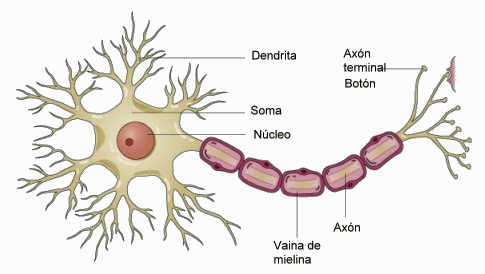
\includegraphics[width=11cm]{./RedNeuronalBiologica}
\caption{Partes de una neurona biológica.}
\end{center}
\end{figure}

Este punto de unión es el encargado de transferir los impulsos eléctricos generados en la membrana de la neurona. Esta información viaja a través de los axones en breves impulsos eléctricos.\\

El conjunto de un gran número de neuronas conectadas entre sí forman la llamada red neuronal. Conforman el sistema nervioso y el cerebro: el cerebro humano puede contener 10\textsuperscript{11} neuronas y 10\textsuperscript{15} interconexiones. Las redes neuronales biológicas pueden establecerse como grupos de neuronas activas especializadas en tareas como cálculos matemáticos, posicionamiento y memoria.\\
\end{comment}

\section{Contexto y motivación}
\lhead[\thepage]{\thesection. Contexto y motivación}

El deseo de crear y desarrollar aplicaciones que simulen el comportamiento humano es algo que lleva existiendo desde hace mucho tiempo. Durante las última décadas, ha ido aumentando gradualmente el progreso en la construcción de máquinas inteligentes que puedan ejecutar ciertas tareas tal y como la realizaría un ser humano. Este área se denomina Inteligencia Artificial (IA) \cite{IA_Introduccion}.\\

Para llevar a cabo este propósito, dentro del ámbito de la IA, han surgido varias técnicas como el \textit{Machine Learning} o aprendizaje automático (AA) y más recientemente el \textit{Deep Learning} o aprendizaje profundo (AP) el cual surgió para solucionar las limitaciones que presentaba el AA. El objetivo de estas técnicas es crear algoritmos con los que las máquinas sean capaces de \textit{aprender} ciertos comportamientos.\\

Este trabajo se encuadra en el contexto del AP, con el objetivo de detectar objetos en imágenes. Durante el desarrollo del mismo, y debido a la utilización del \textit{Deep Learning}, se utilizarán las redes neuronales artificiales (RNA), más concretamente el tipo llamado redes neuronales convolucionales (CNN, del inglés \textit{Convolutional Neural Network}), y la técnica \textit{Single Shot MultiBox Detection} (SSD), conceptos que serán explicados y desarrollados más adelante.

\section{Inteligencia artificial y aprendizaje automático}
\lhead[\thepage]{\thesection. Inteligencia artificial y aprendizaje automático}

El concepto de IA no tiene una definición específica. No existe un consenso entre los científicos e ingenieros que tratan el problema de la IA. Tal vez, una de las definiciones que se puede considerar más ajustada es la reflejada en la \textit{Encyclopedia of Artificial Inteligence} \cite{IA_Encyclopedia}:\\

\textbf{La IA es un campo de la ciencia y la ingeniería que se ocupa de la compresión, desde el punto de vista informático, de lo que se denomina comúnmente comportamiento inteligente. También se ocupa de la creación de artefactos que exhiben ese comportamiento.}\\

Tras esta definición, se puede deducir que en el seno de la IA como ciencia y tecnología se han ido acumulando conocimientos sobre cómo emular las diversas capacidades del ser humano para exhibir comportamientos inteligentes y se han desarrollado sistemas cada vez más perfeccionados que reproducen parcialmente dichas capacidades \cite{IA}.\\

Para cubrir este objetivo, la IA abarca varios campos de aplicación. A continuación se explican brevemente algunas de las áreas más importante donde se aplica \cite{IA_2}:
\begin{itemize}
\item \textbf{Tratamiento de lenguajes naturales:} Este campo abarca aplicaciones que realicen traducciones entre idiomas, interfaces hombre-máquina que permitan consultar una base de datos o dar órdenes a un sistema operativo que permita una comunicación más amigable y fluida con el usuario.
\item \textbf{Sistemas expertos:} Aquí se engloban aquellos sistemas dónde la experiencia de personal cualificado se incorpora a dichos sistemas para conseguir deducciones más cercanas a la realidad.
\item \textbf{Robótica:} Navegación de robots móvil, conducción autónoma, ensamblaje de piezas...
\item \textbf{Visión Artificial:} Abarca aplicaciones desarrolladas para reconocimiento de objetos, detección de defectos en piezas por medio de la visión o apoyo en diagnósticos médicos.
\item \textbf{Aprendizaje:} Modelización de conductas para su posterior implantación en computadoras.  
\end{itemize}

Dentro de la IA, surge un nuevo concepto denominado \textit{Machine Learning} o aprendizaje automático (AA). El AA es una disciplina científica del ámbito de la IA cuyo objetivo es desarrollar técnicas que permitan a las computadoras aprender automáticamente. Más concretamente, se trata de crear aplicaciones capaces de generalizar comportamientos a partir de información suministrada en forma de ejemplos. Se puedes definir, por lo tanto, como un proceso de inducción del conocimiento. Se dice que un sistema tiene la \textit{capacidad de aprender} si adquiere y procesa información acerca de su desempeño y del ambiente que lo rodea, para mejorar dicho desempeño.\\

\begin{figure}[H]
\begin{center}
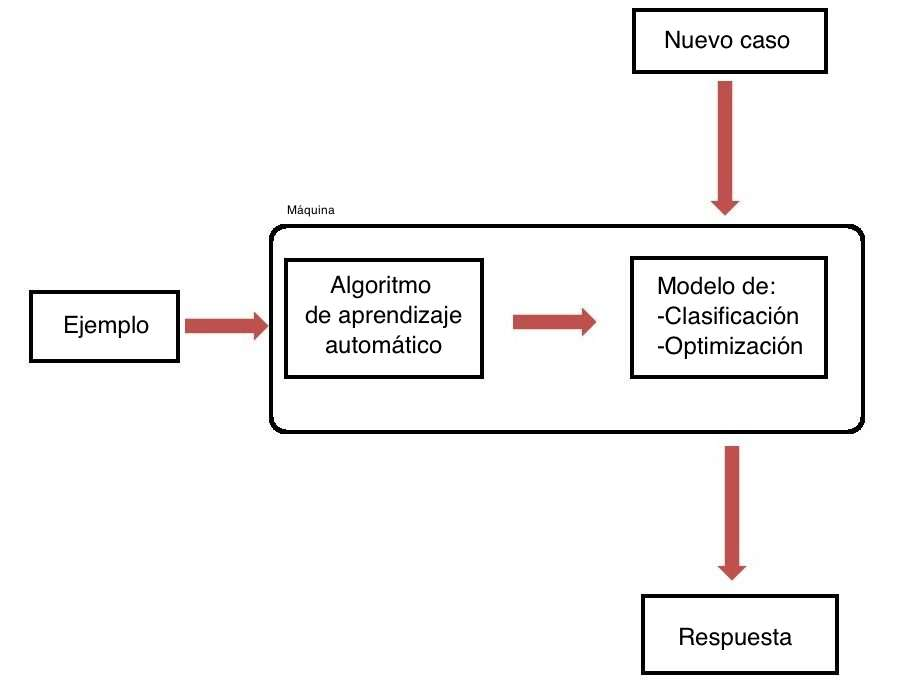
\includegraphics[width=9cm]{./ModeloMachineLearning}
\caption{Modelo Machine Learning. Imagen obtenida de \cite{ML}.}
\label{ModeloMachineLearning}
\end{center}
\end{figure}

\textit{Machine Learning}, se refiere comúnmente a la metodología de aprendizaje automático tradicional, basada en sistemas de decisión lineales y cuyas miles de variantes se llevan utilizando durante años en entornos de computación automatizada.\\

La experiencia ha demostrado que un sistema que utiliza la técnica de \textit{Machine Learning} tradicional donde el número de variables y el volumen de muestras a analizar es demasiado elevado, perderá de manera exponencial precisión y efectividad, necesitando de una gran cantidad de recursos para poder mantener unos tiempos de de decisión aceptables.

\subsection{Aplicaciones}

Actualmente, los grandes avances tecnológicos y las mejores en los algoritmos de AA ha hecho que estas técnicas se utilicen en un gran número de aplicaciones, tanto a nivel de negocio como a nivel de investigación. A continuación, se enumeran algunas de las aplicaciones más importantes desarrolladas o pendientes de desarrollar en el futuro basadas en el AA.

\begin{itemize}
\item \textbf{Conducción autónoma:} El hecho de que un coche pueda ser dirigido sin la acción directa del ser humano es una de las investigaciones más llamativas en el ámbito de la IA. Los investigadores del ámbito de la automoción emplean el AA para detectar automáticamente objetos tales como señales de stop y semáforos. Además, el AA se utiliza para detectar peatones, lo que contribuye a reducir los accidentes.
\item \textbf{Automatización industrial:} El AA está ayudando a mejorar la seguridad de los trabajadores en entornos con maquinaria pesada, gracias a la detección automática de personas u objetos cuando se encuentran a una distancia no segura de las máquinas.
\item \textbf{Electrónica:} El aprendizaje electrónico se usa en la audición automatizada y la traducción del habla. Por ejemplo, los dispositivos de asistencia doméstica que responden a la voz y conocen sus preferencias se basan en aplicaciones de aprendizaje profundo.
\item \textbf{Investigación médica:} En el ámbito de la salud, como por ejemplo al revisar una mamografía, los algoritmos de AA pueden procesar más información y detectar más patrones que una mente humana. Además, el AA también se puede utilizar para advertir los factores de riesgo de enfermedad en poblaciones grandes.
\begin{figure}[H]
\begin{center}
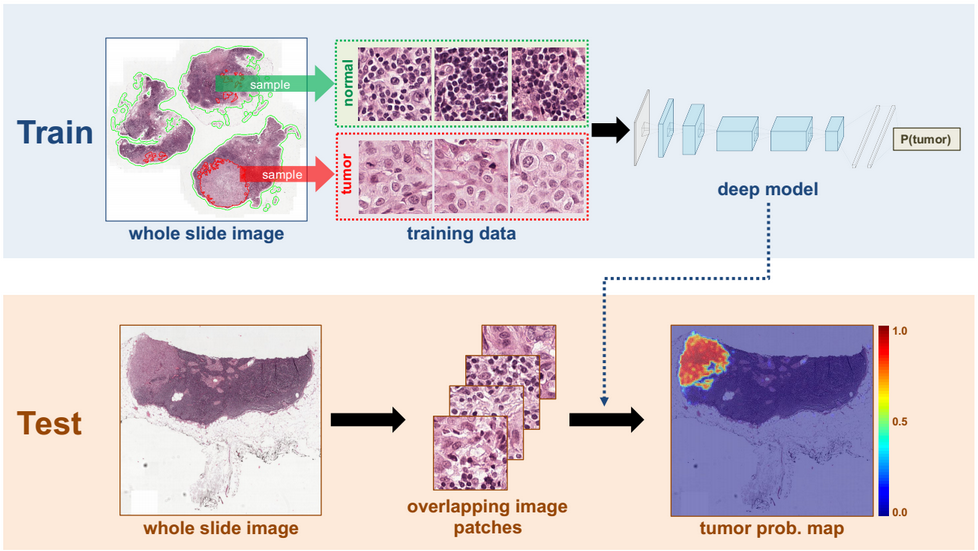
\includegraphics[width=9cm]{./CancerDL}
\caption{Ejemplo de AA aplicado a la detección de cáncer de mama. Imagen obtenida de \cite{CancerMamaDeepLearning}.}
\label{MArcoIA}
\end{center}
\end{figure}
\end{itemize}

\section{Redes neuronales artificiales}
\lhead[\thepage]{\thesection. Redes neuronales artificiales}

Muchas variedades de redes adaptativas han demostrado ser prácticas enfrentándose a problemas de gran dificultad, convirtiendo el estudio de sus propiedades matemáticas y computacionales en un campo muy interesante de estudio.\\

Por ello, a partir de las redes neuronales biológicas, se crean las redes neuronales artificiales (RNA) las cuales son modelos simplificados de las redes neuronales biológicas. Tratan de imitar las capacidades del cerebro para resolver ciertos problemas complejos como reconocimiento de patrones o control moto-sensorial.\\

Consisten en un gran número de elementos simples de procesamiento llamados nodos o neuronas que están organizados en capas. En el modelo de una neurona artificial, representado en la figura \ref{ModeloRedNeuronal}, se pueden identificar varios elementos.

\begin{itemize}
\item \textbf{Enlaces de conexión:} Parametrizados por los pesos sinápticos \textit{w\textsubscript{n}}. Si \textit{w\textsubscript{n}} \textgreater 0 la conexión es excitadora mientras que si \textit{w\textsubscript{n}} \textless 0, la conexión será inhibidora.
\item \textbf{Sumador:} Suma los componentes de las señales de entrada multiplicadas por los pesos sinápticos \textit{w\textsubscript{n}}.
\item \textbf{Función de activación:}  Transformación no lineal del sumatorio obtenido.
\end{itemize}

\begin{figure}[H]
\begin{center}
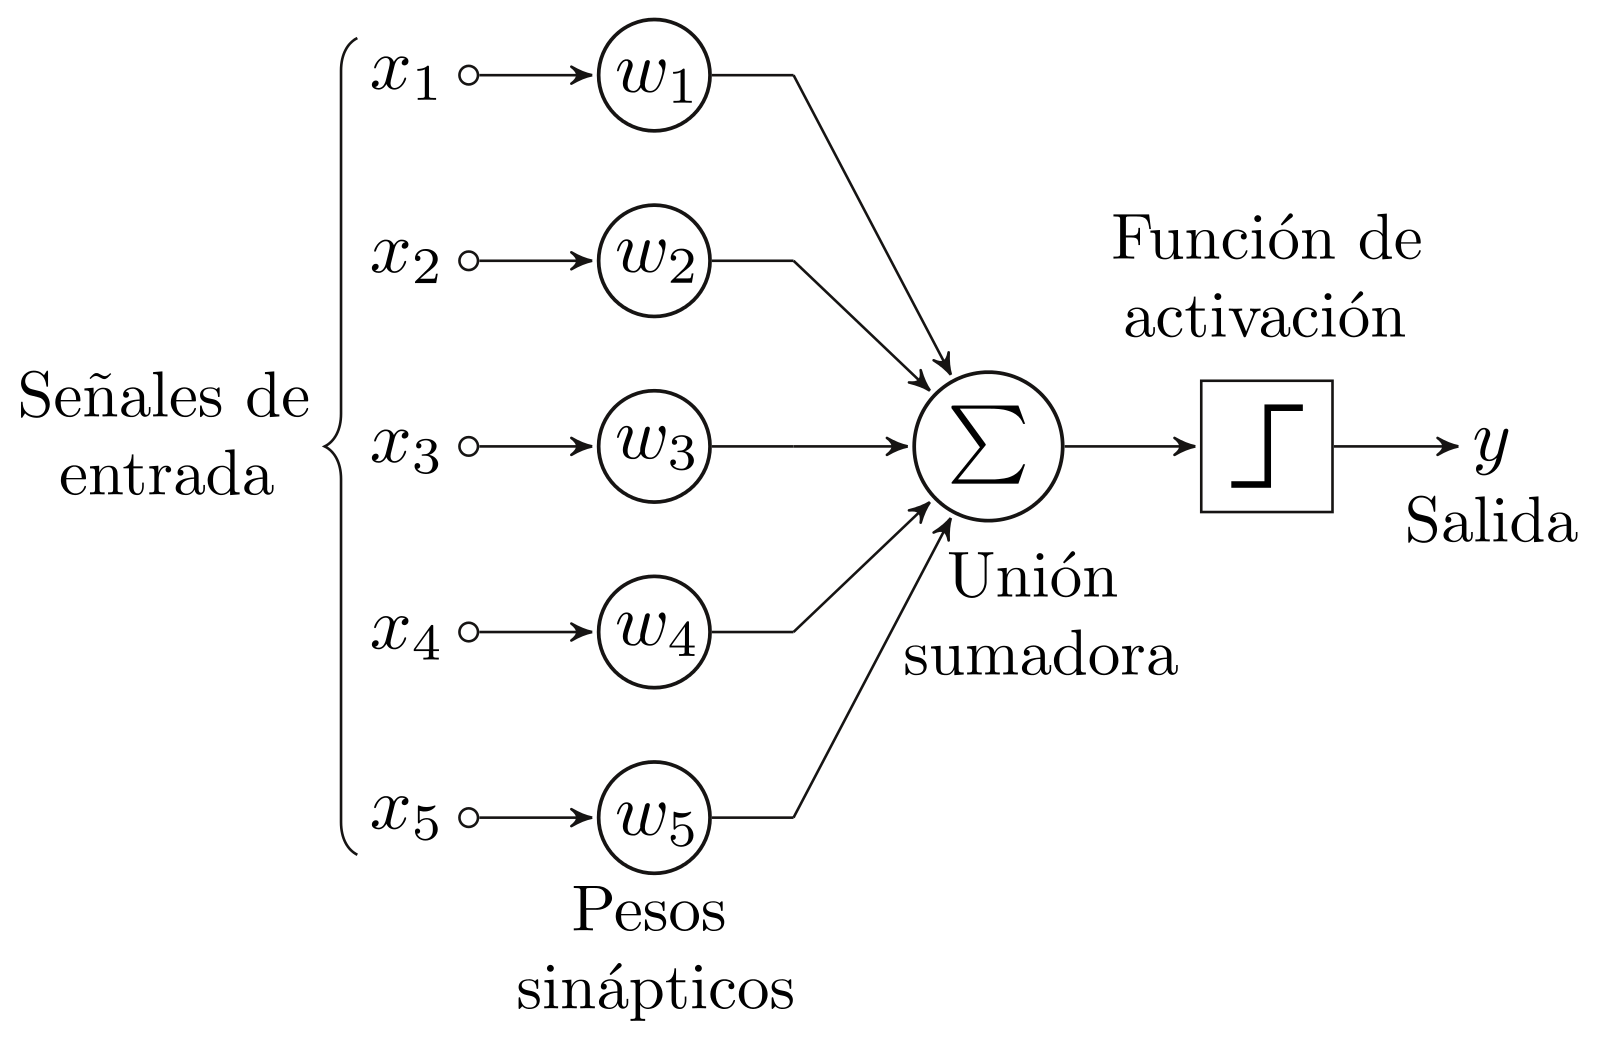
\includegraphics[width=11cm]{./ModeloRedNeuronal}
\caption{Modelo de una neurona artificial. Imagen obtenida de \cite{NeuronaModelo}.}
\label{ModeloRedNeuronal}
\end{center}
\end{figure}

Para definir totalmente una RNA, hay que especificar el conexionado existentes entre cada una de las neuronas que lo forman. Éstas se agrupan en capas, cada una de ellas con un número de neuronas variable y comportamiento similar, constituyendo varias capas de una red neuronal.\\

Cada capa está conectada total o parcialmente a la que se encuentra inmediatamente después, excepto la última capa, que constituye la salida total de la red neuronal. Existen 3 tipos de capas \cite{TiposCapasRNA}:

\begin{itemize}
\item \textbf{Capa de entrada:} También denominada capa sensorial, está compuesta por neuronas que reciben datos o señales procedentes del entorno.
\item \textbf{Capas ocultas:} Este tipo de capas no tienen conexión directa con el entorno. Proporcionan grados de libertad a la red neuronal gracias a los cuales es capaz de representar de forma más exacta determinadas características del entorno que trata de modelar.
\item \textbf{Capa de salida:} Está compuesta por neuronas que proporcionan la respuesta de la red neuronal.
\end{itemize}

\begin{figure}[H]
\begin{center}
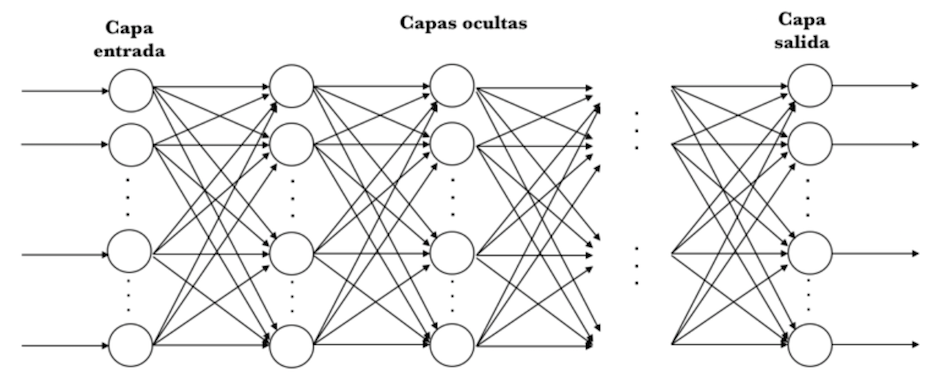
\includegraphics[width=14cm]{./ModeloRNA}
\caption{Modelo de una red neurona artificial. Imagen obtenida de \cite{CapasRNA}.}
\label{ModeloRNA}
\end{center}
\end{figure}

Cada neurona está conectada con otras neuronas mediante enlaces de comunicación, cada uno de los cuales tiene asociado un peso. Los pesos representan la información que será usada por la red neuronal para resolver un problema determinado.\\

Así, las RNA son sistemas adaptativos que aprenden de la experiencia, es decir, aprenden a llevar a cabo ciertas tareas mediante un entrenamiento con ejemplos ilustrativos. Mediante este entrenamiento o aprendizaje, las redes neuronales artificiales crean su propia representación interna del problema. Posteriormente, pueden responder adecuadamente cuando se les presentan situaciones a las que no habían sido expuestas anteriormente, es decir, las RNA son capaces de generalizar de casos anteriores a casos nuevos.

\subsection{Aprendizaje en redes neuronales artificiales}

Tras definir la arquitectura, el siguiente paso es el entrenamiento o aprendizaje. El conocimiento de una red neuronal se encuentra distribuido en los pesos de las conexiones existentes entre todas las conexiones de la red. La red neuronal aprende variando el valor de sus parámetros, en particular los pesos sinápticos y el umbral de polarización. El aprendizaje es un proceso por el cual los parámetros se adaptan por la iteración continua con el medio ambiente. El tipo de aprendizaje está determinado por la forma en que se realiza dicha adaptación. Este proceso implica la siguiente secuencia de eventos:

\begin{itemize}
\item La red neuronal es estimulada por el medio ambiente.
\item La red neuronal ajusta sus parámetros
\item La red neuronal genera una nueva respuesta.
\end{itemize}

Actualmente, existen varios criterios, llamados de forma genérica reglas de aprendizaje, para modificar los pesos de la red y así conseguir que aprenda a solucionar un determinado problema. Las reglas de aprendizaje consisten generalmente en algoritmos matemáticos que pueden llegar a ser sumamente complejos. Se suelen considerar dos tipos de reglas de aprendizaje: aprendizaje supervisado y aprendizaje no supervisado.

\begin{itemize}
\item En el aprendizaje supervisado existe un supervisor que controla el proceso de aprendizaje de la red. El supervisor comprueba la salida de la red en respuesta a una determinada entrada y en el caso de que la salida no coincida con la deseada, se procede a modificar los pesos de las conexiones, con el fin de conseguir que la salida obtenida se aproxime a la deseada.
\item Con el aprendizaje no supervisado, también llamado autoorganizado, la red no requiere influencia de un supervisor para ajustar los pesos de las conexiones entre sus neuronas. La red no recibe ninguna información por parte del entorno que le indique si salida generada en respuesta a una determinada entrada es o no correcta. Su función consiste en encontrar las características, regularidades o categorías que se puedan establecer entre los datos que se presentan en su entrada.
\end{itemize}

Una vez obtenidos y guardados los pesos óptimos en la fase de entrenamiento, es necesario medir la eficacia de la red de forma objetiva mediante la presentación de casos nuevos, es decir, entradas diferentes a los casos de entrenamiento, de forma que a la fase de entrenamiento le debe seguir una fase de test. En esta fase no se modifican los pesos, simplemente se presentan casos nuevos, llamados casos de test, a la entrada de la red y ésta proporciona una salida para cada uno de ellos. Si se comprueba que se siguen obteniendo resultados dentro del margen de error deseado, se puede proceder a emplear la red neuronal dentro de su entorno de trabajo real.

\subsection{Redes neuronales convolucionales}\label{CNN_section}

\begin{comment}
Uno de los tipos más populares de redes neuronales profundas son las conocidas como redes neuronales convolucionales (CNN). Las CNN eliminan la necesidad de una extracción de características manual, por lo que no es necesario identificar las características utilizadas para clasificar las imágenes. La CNN funciona mediante la extracción de características directamente de las imágenes. Las características relevantes no se entrenan previamente; se aprenden mientras la red se entrena con una colección de imágenes.\\
\end{comment}

Una CNN, es uno de los tipos de RNA más utilizadas en el ámbito de la IA, más específicamente del reconocimiento de patrones, como por ejemplo visión artificial o reconocimiento de voz.\\

La idea básica de las CNN es construir propiedades de invarianza en redes neuronales mediante la creación de modelos invariables para ciertas transformaciones en la entrada.\\

Para ello, las CNN utilizan una arquitectura especial, mostrada en la figura \ref{ModeloCNN} y compuesta de una capa de convolución y otra de submuestreo. La capa de convolución implementa la función de convolución, mientras que en la capa de submuestreo se realiza el \textit{pooling}, que se encarga de generar características invariantes calculando estadísticas de las activaciones de convolución a partir de un pequeño campo receptivo. 

\begin{figure}[H]
\begin{center}
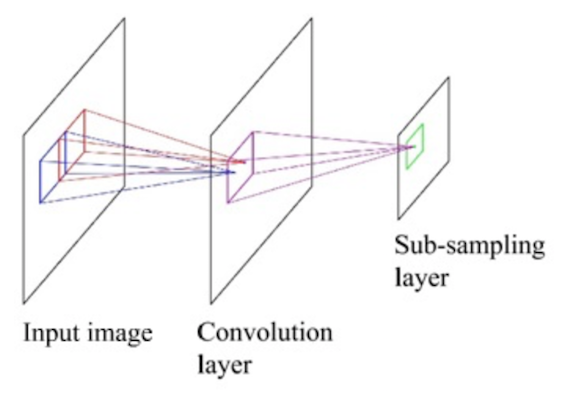
\includegraphics[width=8cm]{./CNN}
\caption{Modelo de una red neurona convolucional. Imagen obtenida de \cite{CNN}.}
\label{ModeloCNN}
\end{center}
\end{figure}

En las CNN, cada neurona de la capa oculta está conectada a un pequeño campo de la capa anterior, el cual será llamado campo receptivo. En la capa de convolución, las neuronas están organizadas en múltiples capas ocultas paralelas, llamadas mapas de características,  de tal manera que cada neurona en un mapa de características está conectada a un campo receptivo local. Para cada mapa de características, todas las neuronas comparten el mismo parámetro de peso que se conoce como filtro o kernel \cite{CNN}.

\begin{figure}[H]
\begin{center}
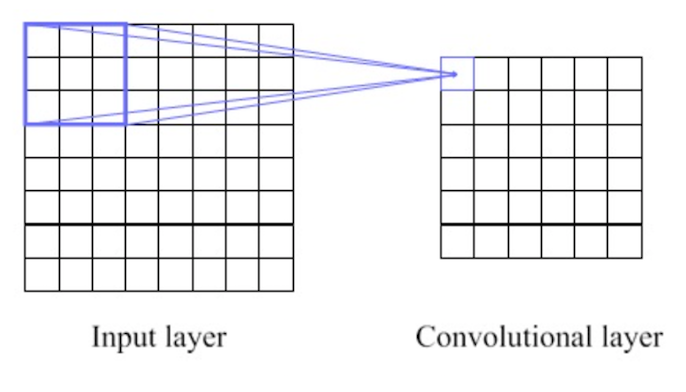
\includegraphics[width=9cm]{./CNN_ConvolutionLayer}
\caption{Ejemplo de campo receptivo local en la capa convolucional. Imagen obtenida de \cite{CNN}.}
\label{CNN_ConvolutionLayer}
\end{center}
\end{figure}

\subsection{Entornos software para redes neuronales}\label{SoftwaresRNN}

Actualmente, el incipiente interés que hay en crear aplicaciones basadas en la inteligencia artificial ha hecho que existan una gran cantidad librerías que permiten desarrollar este tipo de trabajos e investigaciones.\\

A continuación se definen brevemente algunos de los softwares más utilizados para aplicaciones de aprendizaje máquina en la actualidad.

\begin{itemize}
\item Uno de los softwares más populares y extendidos actualmente es la plataforma llamada \textit{Caffe}. Este trabajo ha sido desarrollado utilizando este software, por lo que se detallarán sus características principales más adelante.
\item \textbf{TensorFlow} es una biblioteca software de código abierto diseñada para el cálculo numérico de alto rendimiento. Su arquitectura flexible permite una fácil implementación de computación en una gran variedad de plataformas, tales como CPUs ó GPs, y desde escritorios hasta clústeres de servidores y dispositivos móviles y periféricos. Fue diseñado originalmente por investigadores e ingenieros de Google. Este software cuenta con un sólido soporte para el aprendizaje automático y el aprendizaje profundo y el flexible núcleo de computación numérica del que dispone hace que puede ser utilizado en muchos otros dominios científicos.

\item \textbf{Keras} es una API de redes neuronales de alto nivel escrita en Python y capaz de ejecutarse sobre TensorFlow, CNTK o Theano. Fue desarrolla con el objetivo principal de permitir una experimentación rápida. El enfoque de este software es que el poder pasar de la idea al resultado en el menor tiempo posible es la clave para hacer una buena experimentación.\\

Las características y ventajas principales que pueden definir a esta librería se definen a continuación.

\begin{itemize}
\item \textbf{Facilidad de uso:} Keras es una API diseñada para seres humanos, no para máquinas. Sigue las mejores prácticas para reducir la carga cognitiva: ofrece APIs consistentes y simples, las cuales minimizan el número de acciones de usuario requeridas para casos de uso común y proporciona comentarios claros y procesables ante el error del usuario.
\item \textbf{Modularidad:} Un modelo se entiende como una secuencia o un gráfico de módulos independientes y completamente configurables que se pueden conectar con la menor cantidad de restricciones posible. En particular, las capas neuronales, las funciones de costos, los optimizadores, los esquemas de inicialización, las funciones de activación y los esquemas de regularización se tratan de módulos independientes que se puede combinar para crear nuevos modelos.
\item \textbf{Facilmente extensible:} Los nuevos módulos son simples de agregar, ya sea como nuevas clases o como funciones. Al crearlos se permite una total expresividad, lo que hace de Keras una librería altamente adecuada para la investigación avanzada.
\item \textbf{Trabaja con Python:} No hay archivos de configuración de modelos definidos en un formato declarativo. Los modelos se escriben en código de Python, el cual permite fácilmente la extensión y es compacto y fácil de depurar.
\end{itemize}
\item \textbf{Darknet :} Se trata de un framework de código abierto de redes neuronales escrito en C y CUDA. En su página web oficial\footnote{\url{https://pjreddie.com/darknet/}} se pueden observar varios de los trabajos desarrollados por sus creadores. Algunos de los más destacados son su componente detector en tiempo real, utilizando para el entrenamiento de la red la base de datos COCO, la cual se utilizará en este trabajo, y su clasificador de imágenes para el reto 1000-class ImageNet.
\end{itemize}


\section{Deep Learning}
\lhead[\thepage]{\thesection. Deep Learning}

Como solución a los problemas que presenta el aprendizaje automático, surge el término de \textit{Deep Learning} o aprendizaje profundo (AP) y es entonces cuando tanto este término como el de \textit{Machine Learning} toman mayor relevancia. Por lo tanto, el AP es un conjunto de algoritmos que pertenecen a la clase AA que intentan modelar abstracciones de alto nivel usando arquitecturas compuestas de transformaciones no lineales múltiples.\\

Se pueden relacionar fácilmente los ámbitos del aprendizaje profundo y las redes neuronales. Las redes neuronales artificiales son un paradigma de aprendizaje automático inspirado en las neuronas de los sistemas nerviosos biológicos.\\

La mayor parte de los métodos de aprendizaje emplean arquitecturas de redes neuronales, por lo que, a menudo, los modelos de aprendizaje profundo se denominan redes neuronales profundas. Unas de las RNA más utilizadas en el AP son las CNN, explicadas en el apartado \ref{CNN_section}.En el contexto de la detección de imágenes, que es donde se encuadra este TFG, las CNN resultan idóneas ya que con ésta técnica se procesa cada imagen por secciones en lugar de tener un parámetro por cada píxel de ésta.\\

El término profundo suele hacer referencia al número de capas ocultas en la red neuronal. Las redes neuronales tradicionales solo contienen dos o tres capas ocultas, mientras que las redes profundas pueden tener hasta 150.\\

La gran precisión que se consigue utilizando técnicas de \textit{Deep Learning} contribuye a que se satisfagan las expectativas de los usuarios, y resulta crucial en aplicaciones críticas para la seguridad, tales como los vehículos sin conductor. Los últimos avances en el ámbito del aprendizaje profundo han llegado a un punto en el que este supera a las personas en algunas tareas, como por ejemplo, en la clasificación de objetos presentes en imágenes, lo cual tiene una gran importancia en el ámbito de la medicina, ya que con estas técnicas se pueden detectar, por ejemplo en radiografías, elementos que habían sido obviados por el ser humano.\\

El AP es una forma especializada de AA. Un flujo de trabajo de AA comienza por la extracción manual de las características relevantes de la imagen. Estas características se utilizan entonces para crear un modelo que categoriza los objetos de la imagen. Con un flujo de trabajo de AP, las características relevantes se extraen directamente de la imagen.\\

\begin{figure}[H]
\begin{center}
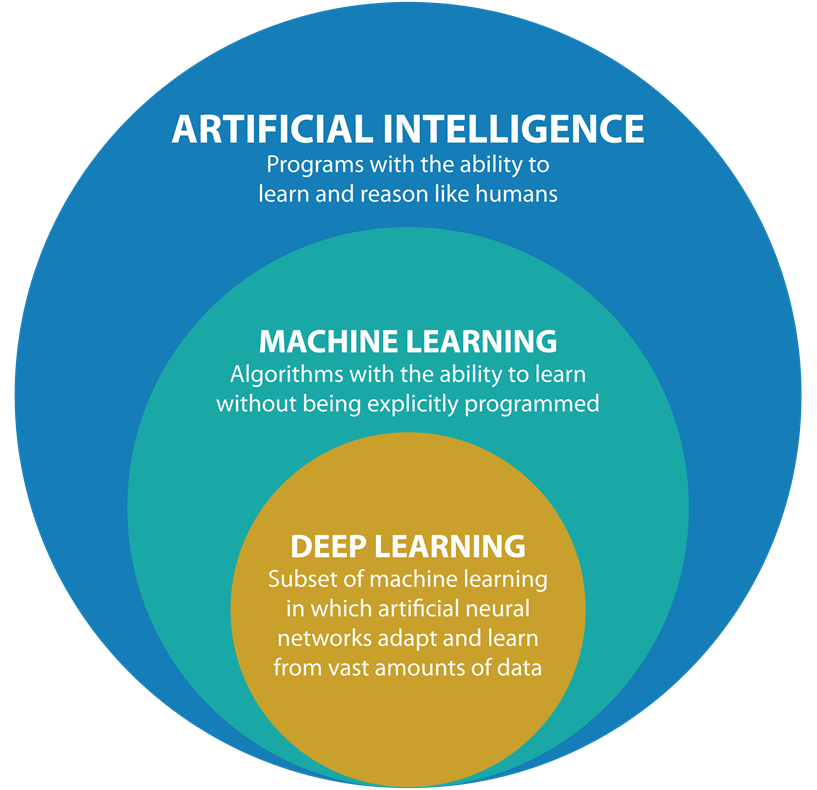
\includegraphics[width=8cm]{./MarcoIA}
\caption{Marco de la Inteligencia Artificial.}
\label{MArcoIA}
\end{center}
\end{figure}

Otra diferencia clave es que con los algoritmos de AP la escala aumenta con los datos, mientras que, en el caso del aprendizaje superficial, existe convergencia. El aprendizaje superficial hace referencia a los métodos de AA que llegan a un punto muerto en cierto nivel de rendimiento cuando se agregan más ejemplos y datos de entrenamiento a la red.\\

Una ventaja fundamental de las redes de aprendizaje profundo es que suelen seguir mejorando a medida que aumenta el tamaño de los datos.\\

\begin{figure}[H]
\begin{center}
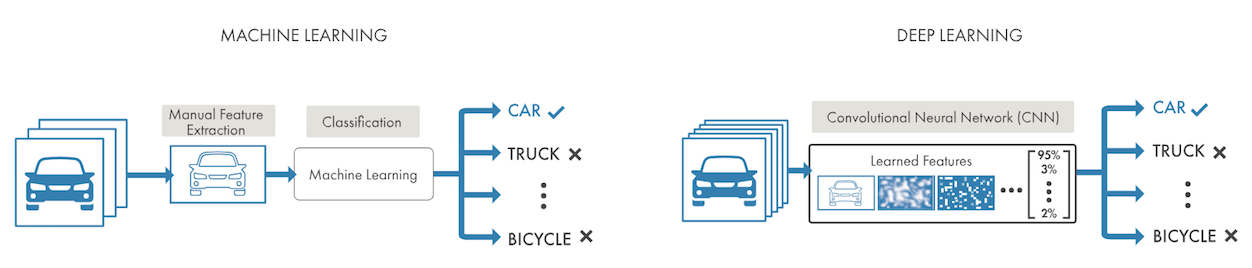
\includegraphics[width=14cm]{./MLvsDL}
\caption{Comparación de un enfoque de aprendizaje automático para la categorización de vehículos (izquierda) con el aprendizaje profundo (derecha). Imagen obtenida de \cite{SSD_3}.}
\label{MArcoIA}
\end{center}
\end{figure}


\section{Antecedentes en el proyecto JdeRobot}
\lhead[\thepage]{\thesection. ANTECEDENTES JDEROBOT}

Actualmente, en JdeRobot ya se han desarrollado varios trabajos basados en la inteligencia artificial y más concretamente en deep learning. En ellos se han utilizado algunos de los softwares mencionados anteriormente para entrenar una o varias redes neuronales. Tras ello, se han abordado tareas de clasificación y detección de objetos analizando tras ellos la capacidad que tenían las redes neuronales ya entrenadas para realizar ese cometido.\\

Nuria Oyaga\footnote{\url{https://jderobot.org/Noyaga-tfg}} realizó un trabajo basado en la clasificación de dígitos manuscritos. Para el estudio y utilización de las redes neuronales usó la plataforma \textit{Caffe}, la cual provee de una red básica ideal para  comenzar en el campo de la clasificación.\\

Como banco de imágenes de entrada, cuyo objetivo es entrenar la red neuronal, utilizó  Modified National Institute of Standards and Technology (MNIST). Esta base de datos está constituida por números escritos a mano y consta de un conjunto de entrenamiento de 60.000 ejemplos y otro de prueba de 10.000. Estas imágenes están dispuestas en escala de grises.\\

\begin{figure}[H]
\begin{center}
\subfloat[]{
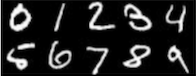
\includegraphics[width=5cm]{./MNIST}}
\subfloat[]{
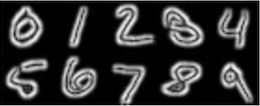
\includegraphics[width=5cm]{./SobelMNIST}}
\caption{(a) Muestras de la base de datos MNIST. (b) Muestras de imágenes aplicando el filtro Sobel.}
\label{MNIST}
\end{center}
\end{figure}

Para evaluar el rendimiento del clasificador, modificó la base de datos MNIST realizando transformaciones sobre sus imágenes y utilizándolas posteriormente para entrenar la red neuronal. Algunas de estas transformaciones fueron la inclusión de filtros a los ejemplos, tales como el Laplaciano, Sobel o Canny y modificaciones basadas en el escalado, translación y rotación de las imágenes de entrada.\\

Además de la evaluación de prestaciones de la red, Nuria realizó un componente para la clasificación de dígitos manuscritos en tiempo real. En el presente trabajo se ha realizado una aproximación de este componente pero con la diferencia de que el objetivo de éste será la detección de objetos.

\begin{figure}[H]
\begin{center}
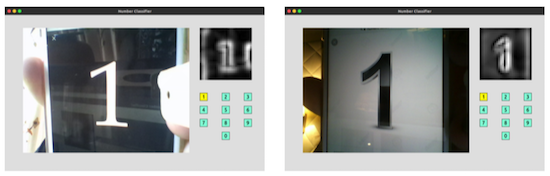
\includegraphics[width=13cm]{./ComponenteClasificador}
\caption{Ejemplo del componente clasificador.}
\label{ComponenteClasificador}
\end{center}
\end{figure}

\begin{comment}
Finalmente, Nuria proporciona la información necesaria para abordar el problema de la detección con Caffe. Muestra algunas pruebas realizadas para la mejor compresión de este proceso. El actual trabajo se centrará en la tarea de detección apoyándose en este primer paso dado por Nuria.\\
\end{comment}

Por otra parte, David Pascual\footnote{\url{https://jderobot.org/Dpascual-tfg}}, realizó un trabajo basado en la clasificación de dígitos manuscritos utilizando la plataforma Keras. Para ello, emplea un modelo proporcionado por éste software y lo entrena utilizando la base de datos MNIST. Además, evalúa las prestaciones de la red realizando una serie de transformaciones sobre los ejemplos de los dígitos y crea un componente para la clasificación de números en tiempo real.\\

\begin{figure}[H]
\begin{center}
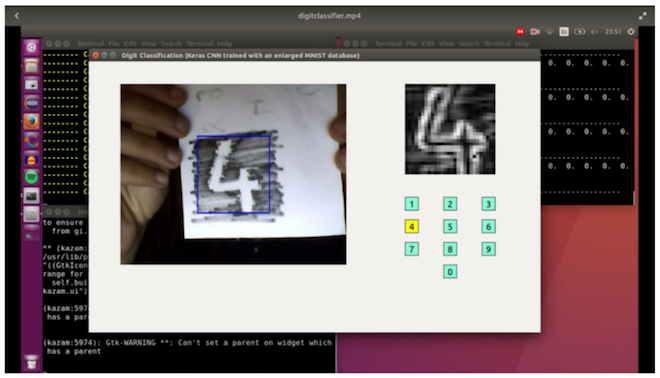
\includegraphics[width=13cm]{./ComponentKeras}
\caption{Ejemplo del componente clasificador.}
\label{ComponentKeras}
\end{center}
\end{figure}

En lo referente a la detección de objetos, en JdeRobot también se han desarrollado varios proyectos. En primer lugar, se puede destacar \textit{DeepLearning Suite}\footnote{\url{https://github.com/JdeRobot/dl-DetectionSuite}} que se trata de un conjunto de herramientas que simplifican la evaluación de los conjuntos de datos de detección de objetos más comunes con varias redes neuronales de detección de objetos.\\

La idea principal es ofrecer una infraestructura genérica para evaluar los algoritmos de detección de objetos contra un conjunto de datos y calcular las estadísticas más comunes, tales como \textit{Intersecion Over Union}, \textit{precision} y \textit{recall}. Esta herramienta acepta un gran número de bases de datos internacionales como PascalVOC y permite la comparación de varias arquitecturas de \textit{Deep Learning} utilizando exactamente la misma prueba.

\begin{figure}[H]
\begin{center}
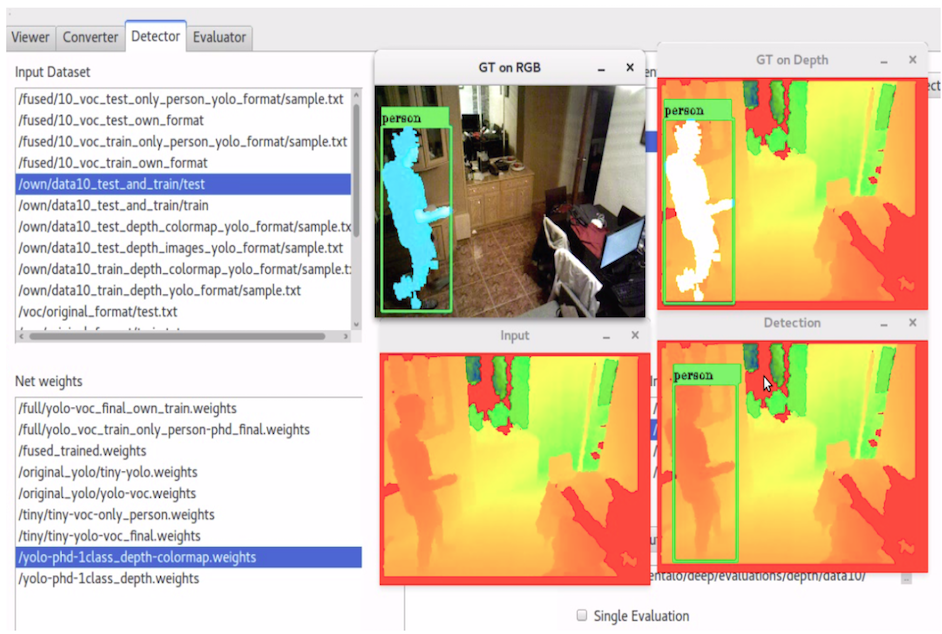
\includegraphics[width=13cm]{./DetectionSuite}
\caption{Herramienta DetectionSuite.}
\label{DetectionSuite}
\end{center}
\end{figure}

Además, Nacho Condés\footnote{\url{https://jderobot.org/Naxvm-tfg}} ha desarrollado un componente de detección de objetos en tiempo real llamado \textit{dl-objectdetector}\footnote{\url{https://github.com/JdeRobot/dl-objectdetector}}. Este componente soporta tanto \textit{Keras} como \textit{TensorFlow} y está escrito en \textit{Python}.

\section{Objetivos}\label{Objetivos}
\lhead[\thepage]{\thesection. OBJETIVOS}

El objetivo principal de este proyecto es el entendimiento de las redes neuronales y el Aprendizaje Profundo o Deep Learning aplicado al problema de la detección de objetos. A partir de lo desarrollado y estudiado durante este trabajo, se pueden identificar varios subobjetivos necesarios para conseguir el objetivo principal. 

\begin{itemize}
\item \textbf{Estudio de la plataforma Caffe:} Se definen en un primer lugar sus principales características y posteriormente se utiliza para el entrenamiento de una red neuronal.
\item \textbf{Estudio de varias bases de datos aplicadas a la detección,} la distribución de los diferentes objetos dentro de sus imágenes y el formato de sus ficheros de anotaciones.
\item \textbf{Estudio de la técnica SSD: } Se definen las principales características de esta técnica en su aplicación en la detección de objetos y posteriormente se integra con Caffe para realizar casos prácticos.
\item \textbf{Desarrollo de un componente detector} que sea capaz de localizar los objetos existentes en las imágenes captadas por una cámara en tiempo real.
\item \textbf{Creación de una base de datos personalizada:} A partir de bases de datos predefinidas, se creará una adicional que contendrá la información de todas ellas.
\item \textbf{Entrenamiento de una red neuronal:} Utilizando Caffe y la base de datos creada se entrenará un red para posteriormente evaluar sus resultados y compararlos con los de otras red preentrenadas.
\begin{comment}
\item \textbf{Desarrollo de \textit{scripts} para el cáculo \textit{índice Jaccard} o \textit{Intersection Over Union}} utilizando un mismo conjunto de imágenes de prueba sobre una misma red neuronal entrenada con diferentes bases de datos. De esta manera se podrán comparar las prestaciones de cada uno de las redes entrenadas.
\end{comment}
\item \textbf{Estudio del \textit{índice Jaccard} o \textit{Intersection Over Union}:} Se realiza una introducción a esté parámetro, a su cálculo y a su función a la hora de evaluar los resultados redes neuronales entrenadas. Se desarrollan \textit{scripts} orientados al entendimiento y cálculo de este índice.
\item \textbf{Realización de experimentos con la herramienta \textit{Detection Suite}} con el objetivo de comparar las prestaciones de varias redes entrenadas con diferentes bases de datos.
\end{itemize}

\section{Metodología}
\lhead[\thepage]{\thesection. METODOLOGÍA}

Durante el desarrollo de este trabajo se han utilizado varias herramientas que han contribuido a qué la dinámica fuera organizada y cooperativa entre todos los miembros del grupo y a que en todo momento, éstos estuvieran al tanto de todo el material que se iba desarrollando y redactando.\\

La principal herramienta, han sido las reuniones concertadas periódicamente con los tutores, Inmaculada Mora y Jose María Cañas. En éstas, se exponían los avances realizados durante la semana, las dudas surgidas y se exponían y proponían nuevas líneas para el desarrollo del trabajo.\\

Para la organización del código generado se ha utilizado el repositorio \textit{GitHub}\footnote{\url{https://github.com/RoboticsURJC-students/2016-tfg-David-Butragueno}}. En él, se encuentra todo el código desarrollado durante el trabajo, con el objetivo de que pueda ser reutilizado, corregido o modificado en función de las necesidades.\\

Con el objetivo de documentar, semana a semana, todo lo desarrollado, se ha utilizado la \textit{Wiki}\footnote{\url{https://jderobot.org/Davidbutra-tfg}} que proporciona \textit{JdeRobot}. Gracias esto, se podía tener acceso al trabajo realizado semanas atrás y los tutores podían revisar antes de la reunión lo realizado durante la semana, haciendo que ésta fuera más práctica y fluida.

\section{Estructura de la memoria}
\lhead[\thepage]{\thesection. ESTRUCTURA DE LA MEMORIA}

Para organizar todo lo desarrollado y los objetivos conseguidos durante el trabajo, se elabora la memoria, cuya estructura se especifica a continuación:\\

En el \textbf{Capítulo 1. Introducción}, se expone el contexto general del trabajo. Se definen los conceptos de redes neuronales artificiales, \textit{Deep Learning} y algunas de sus aplicaciones más importantes. Además, se exponen la características más importantes de algunos \textit{softwares} especializados en las redes neuronales y se enumeran algunos de los trabajos desarrollados en este campo por el proyecto \textit{JdeRobot}.\\

En el \textbf{Capítulo 2. Infraestructura} se especifican todos los elemento \textit{software} utilizados durante el trabajo, incluyendo la plataforma \textit{Caffe} especializada en redes neuronales, el entorno \textit{JdeRobot} y las bases de datos usadas para el entrenamiento.\\

En el \textbf{Capítulo 3. Detección con Single Shot MultiBox y Caffe}, en un primer lugar se define  de forma amplia y teórica las características principales de la técnica SSD. Finalmente, se muestra un ejemplo de como integrar esta técnica en la plataforma \textit{Caffe}, y se muestra el componente creado cuyo objetivo es la detección de objetos en tiempo real.\\

En el \textbf{Capítulo 4. Medidor de calidad} se medirán las prestaciones de la red entrenad y alguna preentrenada con diferentes bases de datos. Se explicará el concepto de \textit{índice Jaccard} y se describirán detalladamente los \textit{scripts} creados para calcular este parámetro. Finalmente, se realizará una breve introducción a la herramienta \textit{Detection Suite} y se utilizará para evaluar los resultados obtenidos y compararlos, proporcionando posteriormente una explicación detallada a éstos.\\

En el \textbf{Capítulo 5. Conclusiones} se resumen las conclusiones obtenidas a lo largo del trabajo y se establecen algunas posibles líneas futuras de investigación en la línea de lo abordado en este trabajo.

\chapter{Infraestructura}
\markboth{INFRAESTRUCTURA}{INFRAESTRUCTURA}

\section{Caffe}
\lhead[\thepage]{\thesection. Caffe}

Caffe es un framework de aprendizaje profundo desarrollado por Berkeley AI Research (BAIR) y por contribuyentes de la comunidad. Fue creado por Yangqing Jia durante su doctorado en UC Berkeley. Caffe está publicado bajo la licencia BSD 2-Clause.\\

Los puntos que definen a este framework y que lo posicionan frente a otros softwares orientados al mismo objetivo son los siguientes:

\begin{itemize}
\item \textbf{La arquitectura expresiva} de Caffe fomenta la aplicación y la innovación. Los modelos y la optimización se definen por configuración y es posible cambiar del uso entre CPU y GPU modificando un único indicador.
\item \textbf{El código extensible} fomenta el desarrollo activo. En el primer año de Caffe, más de 1000 desarrolladores han participado en el proyecto y ha tenido muchos cambios significativos. Gracias a estos colaboradores, el framework sigue el estado del arte tanto en código como en modelos.
\item \textbf{La velocidad} hace que Caffe sea perfecto para experimentos de investigación e implementación en la industria. Caffe puede procesar más de 60 millones de imágenes al día con una sola GPU \textit{NVIDIA K40*}. Esto significa 4 ms/imagen para el aprendizaje, siendo las versiones más recientes de la biblioteca y el hardware aún más rápidos. Por todo esto, Caffe es una de las implementaciones más rápidas disponibles.
\item \textbf{Comunidad:} Caffe ya impulsa proyectos de investigación académica e incluso aplicaciones industriales a gran escala en visión, voz y multimedia. Todo el código desarrollado por la comunidad se encuentra disponible en su repositorio de \textit{GitHub}\footnote{\url{https://github.com/BVLC/caffe/}}.
\end{itemize}

\subsection{Línea de comandos}

Caffe dispone de una interfaz de línea de comandos llamada \textit{cmdcaffe} la cuál es la herramienta utilizada por este software para el entrenamiento del modelo y el diagnóstico del mismo. Los principales comandos que se pueden ejecutar son:

\begin{itemize}
\item \textbf{Entrenamiento:}  Con el comando \textit{caffe train} es posible aprender modelos desde cero, reanudar el aprendizaje a partir de \textit{snapshots} guardadas y ajustar los modelos a los nuevos datos y tareas.
\item \textbf{Test:} El comando \textit{caffe test} califica los modelos ejecutándolos en la fase de test e informa de la salida de la red como su puntuación. En primer lugar se informa la puntuación por lotes de datos de entrada y finalmente el promedio general. 
\item \textbf{Análisis comparativo:} El comando \textit{caffe time} compara el modelo capa a capa. Esto es util para comprobar el rendimiento del sistema y medir los tiempos de ejecución relativos a los modelos.
\item \textbf{Diagnósticos:} El comando \textit{caffe device\_query} informa de los detalles de la GPU para referencia y comprobación del identificador de los dispositivos disponibles para ser ejecutados en máquinas \textit{multi-GPU}.
\item \textbf{Paralelismo:} El indicador \textit{-gpu} de la herramienta Caffe provee una lista separada por comas de IDs para ejecutar procesos en múltiples GPUs.
\end{itemize}

\subsection{Python}

La interfaz de Python \textit{pycaffe} contiene el módulo de Caffe y sus propios scripts en la ruta caffe/python. Con el comando \textit{import caffe} se importará esta interfaz, pudiendo así cargar diferentes modelos de Caffe, manejar instrucciones de entrada/salida, visualizar redes y numerosas funcionalidades más. Todos los datos y parámetros se encuentran disponibles tanto para lectura como para escritura. Algunas de las tareas que se pueden realizar con está interfaz son:

\begin{itemize}
\item \textbf{caffe.Net} es la interfaz central para cargar, configurar y ejecutar modelos.
\item \textbf{caffe.Classifier y caffe.Detector} proporcionan interfaces para tareas de clasificación y detección.
\item \textbf{caffe.SGDSolver} se trata de la interfaz de resolución.
\item \textbf{caffe.io} maneja funciones de entrada/salida.
\item \textbf{caffe.draw} visualiza las arquitecturas de red.
\end{itemize}

\subsection{Capas de una red neuronal}\label{CapaRedNeuronal}

Para crear un modelo de Caffe es necesario definir la arquitectura del mismo utilizando para ello un archivo de definición de buffer de protocolo (prototxt).\\

Las capas de Caffe y sus parámetros están especificados en la definición del buffer de protocolo para el proyecto, en el archivo caffe.proto\footnote{\url{https://github.com/BVLC/caffe/blob/master/src/caffe/proto/caffe.proto}}.

\subsubsection{Capas de datos}

Los datos entran en Caffe a través de las capas de datos, las cuáles se encuentran en la parte inferior de las redes. Estos datos pueden proceder de bases de datos (LevelDB o LMDB), directamente de la memoria, o, cuando la eficiencia no es crítica, desde archivos en disco en formato HDF5 o formatos de imagen comunes.\\

Este tipo de capas son las encargadas de realizar tareas comunes de preprocesamiento de los datos de entrada, tales como sustracción media o escalado, especificando para ello los parámetros de transformación de la propia capa.\\

Todos los sub-tipos de este tipo de capa, se especifican a continuación:

\begin{itemize}
\item \textbf{Image Data:} Lee imágenes sin procesar.
\item \textbf{Database:} Lee los datos de ficheros LevelLDB o LMDB.
\item \textbf{HDF5 Input:} Lee los datos en formato HDF5 permitiendo que estos tengan dimensiones arbitrarias.
\item \textbf{HDF5 Output:} Escribe datos en formato HDF5
\item \textbf{Input:} Normalmente utilizada para redes que se están siendo desplegadas.
\begin{comment}
\item \textbf{Window Data:}
\end{comment}
\item \textbf{Memory Data:} Lee archivos directamente desde memoria.
\item \textbf{Dummy Data:} Utilizado para datos estáticos.
\end{itemize}

\subsubsection{Capas de visión}\label{CapasVision}

Las capas de visión, generalmente toman imágenes como datos de entradas y generan otras imágenes como salida aunque también pueden tomar datos de otros tipos y dimensiones. Una imagen puede tener un canal de color si se trata de una imagen en escala de grises o 3 canales de color si se trata de una imagen RGB. Pero en este contexto, las características distintivas para el tratamiento de las imágenes de entrada serán la altura y la anchura de las mismas. La mayoría de las capas de visión trabajan aplicando una operación particular sobre alguna región de la entrada para producir una región correspondiente a la salida.\\

Existen varios tipos capas de visión, dónde se pueden destacar los más comunes, listados a continuación:

\begin{itemize}
\item \textbf{Convolution Layer:} Convoluciona la imagen de entrada con un conjunto de filtros. Este proceso transforma la matriz de píxeles de la imagen original en otra matriz de características. Esta nueva imagen es esencialmente la original pero cada píxel tiene mucha más información ya que contiene información de la región en la que se encuentra el píxel, no sólo del píxel aislado.\\

\begin{figure}[H]
\begin{center}
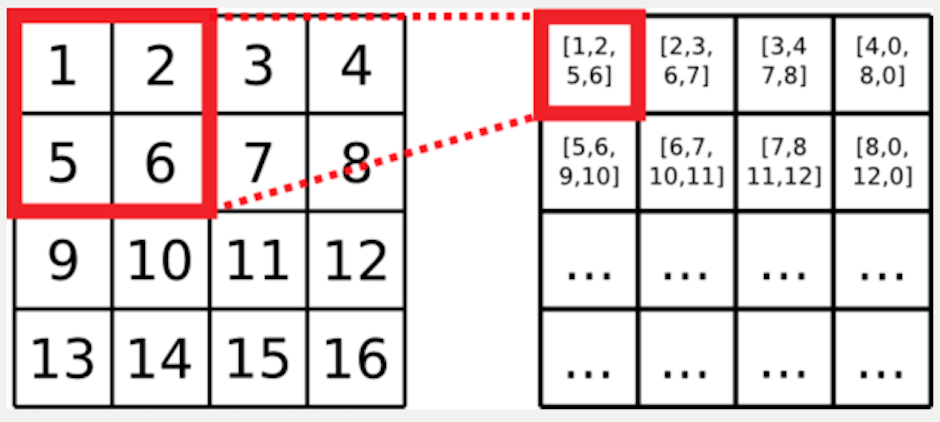
\includegraphics[width=9cm]{./Convolution}
\caption{Ejemplo convolución con tamaño del núcleo 2x2.}
\end{center}
\end{figure}

\item \textbf{Pooling Layer:} Realiza \textit{pooling} de los datos de entrada utilizando para ello funciones de máximo, media o estocásticas. La capa de pooling se coloca generalmente después de la capa de convolución. Su utilidad principal radica en la reducción espacial de la imagen de entrada. Para ello, se divide el mapa de características obtenido anteriormente en un conjunto de bloques de m x n. A continuación, se aplica una función de agrupación para cada uno de los bloques. Tras este proceso, se obtendrá una matriz de características más pequeño. Dentro de las funciones de agrupación, destacan max pooling, el cual elige el valor más alto dentro del bloque y pooling promedio (average) el cual toma como respuesta de bloque el valor promedio de las respuestas del bloque.\\

\begin{figure}[H]
\begin{center}
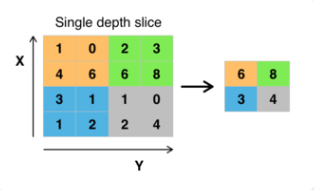
\includegraphics[width=7cm]{./Pooling}
\caption{Pooling con función de agrupación del máximo.}
\end{center}
\end{figure}
\begin{comment}
\item \textbf{Spatial Pyramid Pooling (SPP)} 
\item \textbf{Crop}
\item \textbf{Deconvolution Layer:} Realiza uno convolución transpuesta.
\item \textbf{Im2Col}
\end{comment}
\end{itemize}

\begin{comment}
\subsubsection{Capas recurrentes}

\begin{itemize}
\item \textbf{Recurrent}
\item \textbf{RRNN}
\item \textbf{Long-Short Term Memory (LSTM)}
\end{itemize}
\end{comment}

\subsubsection{Capas comunes}

\begin{itemize}
\item \textbf{Inner Product:} Este tipo de capa trata la entrada como un vector simple y produce una salida en forma de otro vector, estableciendo la altura y la anchura de cada \textit{blob} a 1.
\item \textbf{Dropout}
\item \textbf{Embed}
\end{itemize}

\subsubsection{Capas de pérdida}

Estas capas de pérdida conducen al aprendizaje comparando la salida obtenida con el valor de la entrada asignado así un coste para minimizarla.

\begin{itemize}
\item \textbf{Multinomial Logistic Loss}
\item \textbf{Infogain Loss}
\item \textbf{Softmax with Loss}
\item \textbf{Sum-of-Squares / Euclidean}
\item \textbf{Hinge / Margin}
\item \textbf{Sigmoid Cross-Entropy Loss}
\item \textbf{Accuracy / Top-k layer}
\item \textbf{Contrastive Loss}
\end{itemize}

\subsubsection{Capas de normalización}

\begin{itemize}
\item \textbf{Local Response Normalization (LRN):} Normaliza regiones locales de los datos de entrada.
\item \textbf{Mean Variance Normalization (MVN):} Realiza una normalización de contraste / normalización de instancia.
\item \textbf{Batch Normalization:} Realiza normalizaciones sobre pequeños lotes de datos de entrada.
\end{itemize}

\subsubsection{Capas de activación}\label{CapasActivacion}

En general, estas capas son operados que toman un dato de la salida de la capa anterior y generan datos con las mismas dimensiones.
\\\\

\begin{itemize}
\item \textbf{ReLU / Rectified-Linear and Leaky-ReLU:} Se trata de una función lineal, rectilínea con pendiente uniforme.\\

\begin{figure}[H]
\begin{center}
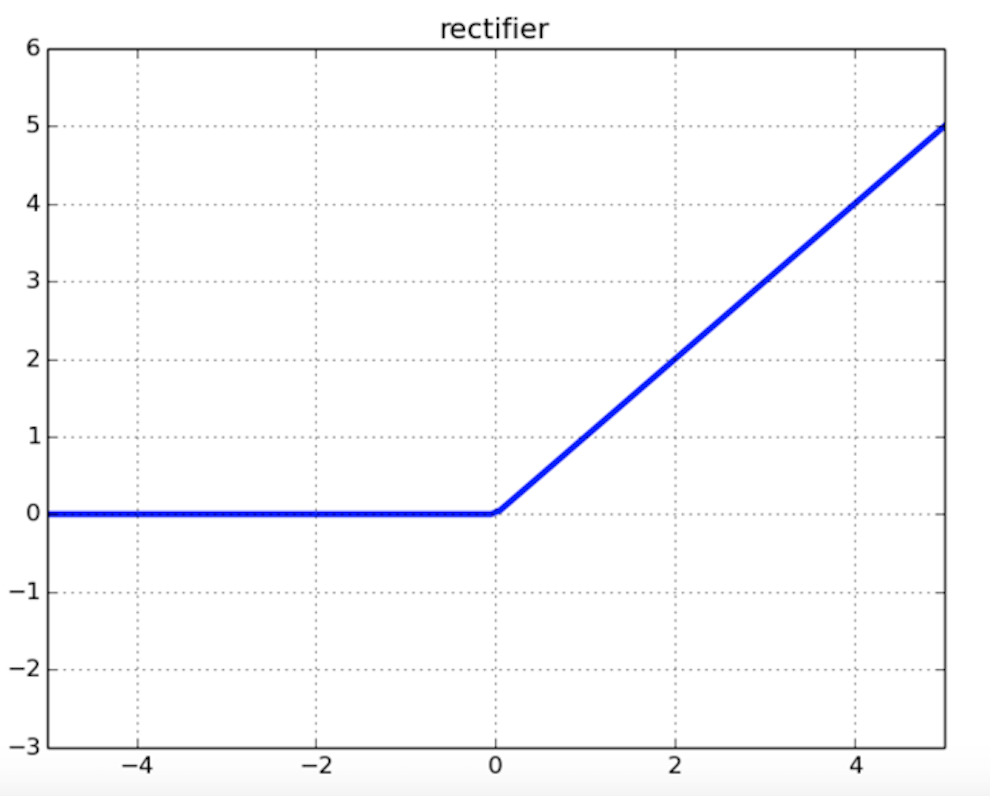
\includegraphics[width=7cm]{./ReLu}
\caption{Función de activación ReLu.}
\end{center}
\end{figure}

Se puede definir a partir de la siguiente ecuación:\\

\begin{equation}
f(x) = \left\lbrace
\begin{array}{ll}
\textup{0 si } x<0\\
\textup{x si } x\geq 0
\end{array}
\right.
\end{equation}

\item \textbf{PReLU}

\item \textbf{ELU}

\item \textbf{Sigmoid}

\begin{figure}[H]
\begin{center}
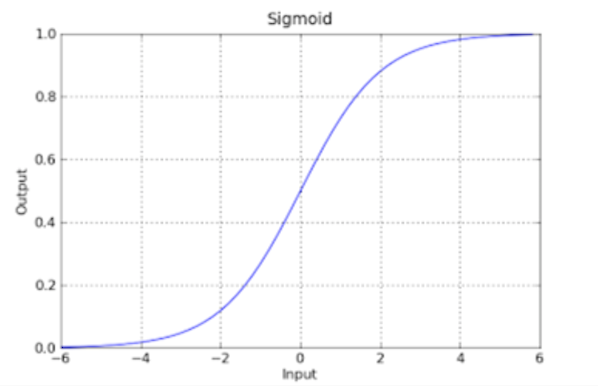
\includegraphics[width=9cm]{./Sigmoid}
\caption{Función de activación Sigmoide.}
\end{center}
\end{figure}

Se puede definir a partir de la siguiente ecuación:\\

\[ f(x)=\frac{1}{1 + e ^ {-x}}\]

\item \textbf{TanH}
\item \textbf{Absolute Value}
\item \textbf{Power} 

\begin{equation}
f(x) = (shift + scale * x) ^ {power}
\end{equation}

\item \textbf{Exp}

\begin{equation}
f(x) = base ^ {(shift + scale * x)}
\end{equation}
\item \textbf{Log}

\begin{equation}
f(x) = log(x)
\end{equation}
\item \textbf{BNLL}

\begin{equation}
f(x) = log(1 + exp(x))
\end{equation}
\\
\item \textbf{Threshold}: Realiza la función de paso en el umbral definido por el usuario.
\item \textbf{Bias} 
\item \textbf{Scale}
\end{itemize}


\section{JdeRobot}
\lhead[\thepage]{\thesection. JdeRobot}

Se trata de un framework cuyo objetivo es desarrollar aplicaciones en robótica y visión por computadora. También tiene actuación en domótica y en escenarios con sensores, accionadores y software inteligente. Ha sido desarrollado para ayudar en la programación de este software inteligente. Está escrito principalmente utilizando el lenguaje C++ proporcionando un entorno de programación en el que el programa de aplicación está compuesto por una colección de varios componentes asíncronos concurrentes. Estos componentes pueden ejecutarse en diferentes equipos y están conectados mediante el middleware de comunicaciones ICE. Los componentes pueden estar escritos en C++, Python, Java y todos ellos ellos interactúan a través de interfaces ICE explícitas.\\

JdeRobot simplifica el acceso a dispositivos hardware desde el programa de control. Obtener mediciones de sensores es tan simple como llamar a una función local y ordenar comandos de motor tan fácil como llamar a otra función local. La plataforma adjunta esas llamadas a invocaciones remotas sobre los componentes conectados al sensor o los dispositivos de accionamiento. También, pueden conectarse a sensores y activadores reales o simulados, tanto a nivel local como remoto utilizando para ello la red. Esas funciones construyen la API para la capa de abstracción del hardware. La aplicación robótica obtiene las lecturas del sensor y ordena los comandos del actuador usando esa API para desplegar su comportamiento. Se han desarrollado varios drivers para soportar diferentes sensores, activadores y simuladores. Los robots y sensores actualmente soportados son:
\\
\begin{itemize}
\item \textbf{Sensores RGBD:} Kinect and Kinect2 de Microsoft, Asus Xtion
\item \textbf{Robots con ruedas:} Kobuki (TurtleBot) de Yujin Robot y Pioneer de MobileRobotics Inc.
\item \textbf{ArDrone quadrotor de Parrot}
\item \textbf{Escáneres laser:} LMS de SICK, URG de Hokuyo y RPLidar
\item \textbf{Simulador Gazebo}
\item \textbf{Cámaras Firewire, cámaras USB, archivos de vídeo (mpeg, avi), cámaras IP (como Axis)}
\end{itemize}

JdeRobot incluye varias herramientas de programación de robots y bibliotecas. En primer lugar, teleespectadores y teleoperadores para varios robots y sus sensores y motores. En segundo lugar, un componente de calibración de cámara y una herramienta de tunning para filtros de color. En tercer lugar, una herramienta llamada VisualHFSM para la programación del comportamiento del robot utilizando la jerarquía Finite State Machines. Además, también proporciona una biblioteca para desarrollar controladores difusos y otra para la geometría proyectiva y el procesamiento de la visión por computadora.
\\

Cada componente puede tener su propia interfaz gráfica de usuario o ninguna en absoluto. Actualmente, las bibliotecas GTK y Qt son compatibles, incluyéndose varios ejemplos de OpenGL para gráficos 3D con ambas bibliotecas.
\\

JdeRobot es un software de código abierto con licencia como GPL y LGPL. También utiliza software de terceros como el simulador Gazebo, ROS, OpenGL, GTK, Qt, Player, Stage, GSL, OpenCV, PCL, Eigen u Ogre.


\subsection{CameraServer}\label{Camera}

Se trata de un componente facilitado por \textit{JdeRobot} que actúa como servidor de imágenes proporcionando a las aplicaciones de estas imágenes procedentes de un número determinado de cámaras, ya sean reales o simuladas, o de un archivo de vídeo.\\

Para el uso correcto de este componente, es necesario editar un fichero de configuración en función de las necesidades concretas de la máquina. En este archivo, con extensión \textit{cfg}, se pueden definir varios parámetros:

\begin{itemize}
\item \textit{EndPoint} del servidor que va a recibir la petición
\item Número de cámaras que se usarán
\item Configuración de las cámaras. Se podrán modificar los siguientes parámetros relacionados con las cámaras:
\begin{itemize}
\item Nombre de la cámara
\item El parámetro URI que define la fuente de vídeo.
\item Numerador y denominador de \textit{frame rate}
\item Formato de la imagen
\item Altura y anchura de las imágenes
\end{itemize}
\end{itemize}

\begin{comment}
\section{Formato de ficheros}

\subsection{eXtensible Markup Language}

\textbf{XML} (eXtensible Markup Language - Lenguaje de Marcas Extensible) es un meta-lenguaje que permite definir lenguajes de marcas, desarrollado por \textit{World Wide Web Consortium} (W3C) y utilizado para almacenar datos de forma legible. A diferencia de otros lenguajes, XML da soporte a bases de datos, siendo útil cuando varias aplicaciones deben comunicarse entre sí o integrar información.\\

XML presenta varias ventajas frente a otros lenguajes, las cuales se definen a continuación:

\begin{itemize}
\item Es extensible, es decir, después de ser diseñado y puesto en producción, es posible la adición de nuevas etiquetas.
\item Mejora la compatibilidad entre aplicaciones. Se pueden comunicar aplicaciones de distintas plataformas sin que importe el origen de los datos.
\item Se transforman datos en información, pues se les añade un significado concreto y y se les asocia a un contexto, con lo cual existe flexibilidad para estructurar documentos.
\end{itemize}

La tecnología XML busca dar solución el problema de expresar información estructurada de la manera más abstracta y reutilizable posible. Que la información sea estructurada quiere decir que se compone de partes bien definidas, y que esas partes, a su vez, se componen de otras partes. De esta forma, surge un árbol de partes de información. Estas partes se llaman \textit{elementos} y vienen definidas mediante \textit{etiquetas}.\\

Una etiqueta consiste en una marca hecha en el documento, que señala una porción de éste como un elemento. Se trata de información con un sentido claro y definido. Las etiquetas tienen la forma <nombre>, donde \textit{nombre} es el nombre del elemento que se está señalando.\\

En la sección \ref{VOC} se puede observar un ejemplo de la estructura de un archivo XML.\\

\subsection{JavaScript Object Notation}

\textbf{JSON} (JavaScript Object Notation - Notación de Objetos de JavaScript) es un formato basado en texto estándar para representar datos estructurados en la sintaxis de objetos de JavaScript. Es comúnmente utilizado para transmitir datos en aplicaciones web, como por ejemplo enviar datos desde el servidor al cliente, haciendo posible que esos datos puedan ser mostrados en páginas web. Aunque es muy parecido a la sintaxis de objeto literal de JavaScript, puede ser utilizado independientemente de éste, y muchos ambientes de programación poseen la capacidad analizar, parsear y generar ficheros JSON.\\

La tecnología JSON tiene varios tipos de datos disponibles, los cuales se presentan a continuación:\\

\begin{itemize}
\item \textbf{Números:} Se permiten números negativos y opcionalmente pueden contener parte fraccional separada por puntos.
\item \textbf{Cadenas:} Representan secuencias de 0 o más caracteres. Se ponen entre dobles comillas.
\item \textbf{Booleanos:} Se permite la representación de valores booleanos.
\item \textbf{Null:} Representa un valor nulo.
\item \textbf{Array:} Representa una lista ordenada de cero o más valores que pueden ser de cualquier tipo. Los valores se separan por comas y el vector se mete entre corchetes.
\item \textbf{Objetos:} Son colecciones no ordenadas de pares \textit{clave:valor} separados por comas y dispuestas entre llaves. La clave tiene que ser una cadena mientras que el valor puede ser de cualquier tipo.
\end{itemize}

En la sección \ref{COCO} se puede observar un ejemplo de la estructura de un archivo JSON.\\

\subsection{Lightning Memory-Mapped Database}

\textbf{LMDB} (Lightning Memory-Mapped Database) es una biblioteca de gestión de bases de datos modelada en la API de BerkeleyDB. Toda la base de datos está modelada como un mapa de memoria, y todos los datos recuperados de ella son datos devueltos directamente de la memoria asignada.\\

La biblioteca es totalmente compatible con subprocesos y admite el acceso simultáneo de lectura y escritura desde múltiples procesos o hilos. Las páginas de datos utilizan una estrategia que permite que no se sobreescriban las páginas con datos activos, lo cual brinda además resistencia a la corrupción de la base de datos. Las escrituras están totalmente serializadas, es decir, solo se permite una escritura de forma simultánea. La estructura de la base de datos tiene múltiples versiones para que las lecturas se ejecuten sin bloqueos; las escrituras sobre ésta no bloquean a las lecturas, y las lecturas no bloquean las escrituras.
\end{comment}

\section{Bases de datos}\label{BBDD}
\lhead[\thepage]{\thesection. Bases de datos}

\subsection{PascalVOC}\label{VOC}

Esta base de datos contiene \textbf{11.530} imágenes de entrenamiento y validación que representan \textbf{27.450} objetos diferentes distribuidos en \textbf{20 clases}. Los datos de entrenamiento proporcionados consisten en un conjunto de imágenes; cada imagen tiene un archivo de anotación que proporciona un cuadro delimitador o \textit{bounding box} y una etiqueta de las 20 clases para cada objeto presente en la imagen. Por lo tanto, la tarea de detección consiste en predecir el cuadro delimitador y la etiqueta de cada objeto en la imagen de prueba.\\

Es importante saber cuántas imágenes aparecen en cada uno de los 20 objetos para saber si la base de datos está bien escalada, o si, por el contrario, algunos objetos aparecen con más frecuencia que otros. En la base de datos VOC2012, las distribuciones de imágenes y objetos por clase son aproximadamente iguales en todos los conjuntos de entrenamiento / validación y prueba. Específicamente, la distribución de objetos para la tarea de detección se muestra en la siguiente imagen.

\begin{figure}[H]
\begin{center}
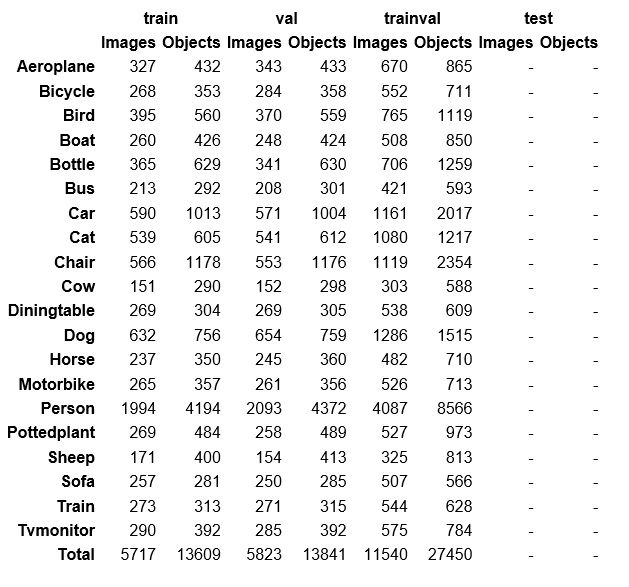
\includegraphics[width=11cm]{./VOC2012_Statics}
\caption{Distribución de objetos en PascalVOC.}
\end{center}
\end{figure}

En cuanto a los archivos de anotaciones, estos tienen un formato XML. En primer lugar, aparecen algunas etiquetas informativas acerca de la imagen, como la etiqueta \textit{filename} que indica el nombre de la imagen, o la etiqueta \textit{database} que indica el nombre de la base de datos.\\

\begin{lstlisting}[frame=single]
	<folder>VOC2012</folder>
	<filename>2007_009084.jpg</filename>
	<source>
		<database>The VOC2007 Database</database>
		<annotation>PASCAL VOC2007</annotation>
		<image>flickr</image>
	</source>
\end{lstlisting}


Después, aparece el grupo de etiquetas \textit{size}, donde se indican el ancho de la imagen, \textit{width}, el alto, \textit{height} y la profundidad, \textit{depth}.\\

\begin{lstlisting}[frame=single]
	<size>
		<width>500</width>
		<height>375</height>
		<depth>3</depth>
	</size>
\end{lstlisting}

Finalmente, aparecen las etiquetas referentes a cada uno de los objetos existentes en la imagen. Destacan la etiqueta \textit{name}, la cual indica el nombre de la etiqueta del objeto, y el grupo \textit{bndbox}, que representa la \textit{bounding box} a partir de las coordenadas \textit{x\_{min}}, \textit{y\_{min}}, \textit{x\_{max}} y \textit{y\_{max}}.\\

\begin{lstlisting}[frame=single]
	<object>
		<name>motorbike</name>
		<pose>Right</pose>
		<truncated>0</truncated>
		<difficult>0</difficult>
		<bndbox>
			<xmin>43</xmin>
			<ymin>77</ymin>
			<xmax>481</xmax>
			<ymax>375</ymax>
		</bndbox>
	</object>
\end{lstlisting}

\subsection{COCO}\label{COCO}

COCO es un conjunto de datos creado para la detección y segmentación de objetos y para generación de subtítulos a gran escala. Algunas de las características de esta base de datos son:

\begin{itemize}
\item Más de 300.000 imágenes
\item 1.5 millones de instancias de objetos
\item 80 categorias de objetos
\end{itemize}

Actualmente, COCO utiliza 3 tipos de anotaciones: instancias de objetos, puntos claves de objetos y leyendas de imágenes. Las anotaciones se almacenan usando el formato de archivo JSON. Todas las anotaciones comparten la estructura de datos básica definida a continuación:

\begin{figure}[H]
\begin{center}
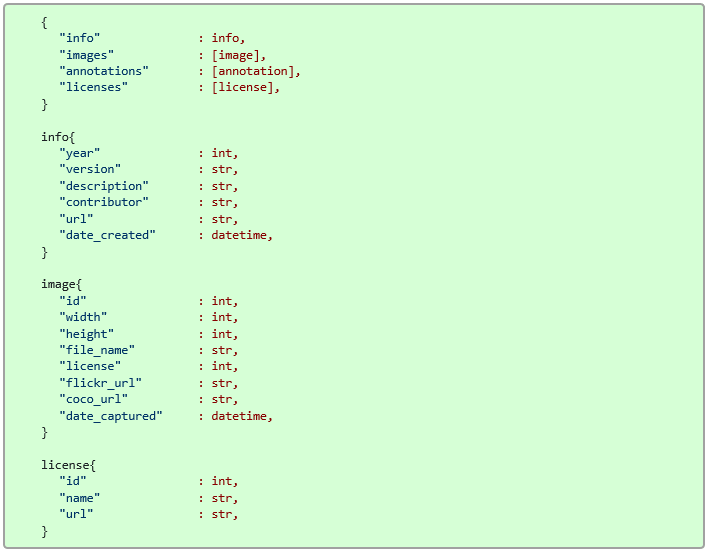
\includegraphics[width=11cm]{./Coco_Annotation_1}
\caption{Estructura básica de anotaciones en COCO.}
\end{center}
\end{figure}

Para la tarea de detección, es de especial interés la anotación usando instancias de objetos. Cada anotación de instancia contiene una serie de campos, incluida la identificación de categoría y la máscara de segmentación del objeto. El formato de segmentación depende de si la instancia representa un solo objeto (\textit{iscrowd = 0} en cuyo caso se usan polígonos) o una colección de objetos (\textit{iscrowd = 1} en cuyo caso se usa RLE). Hay que tener en cuenta que un solo objeto (\textit{iscrowd = 0}) puede requerir múltiples polígonos. Las anotaciones de multitudes (\textit{iscrowd = 1}) se utilizan para etiquetar grandes grupos de objetos, como por ejemplo, una multitud de personas. Además, se proporciona un cuadro delimitador para cada objeto (las coordenadas del cuadro se miden desde la esquina superior izquierda de la imagen y están indexadas en 0). Finalmente, el campo de categorías de la estructura de anotación almacena la asignación de los nombres de categoría y supercategoría.

\begin{figure}[H]
\begin{center}
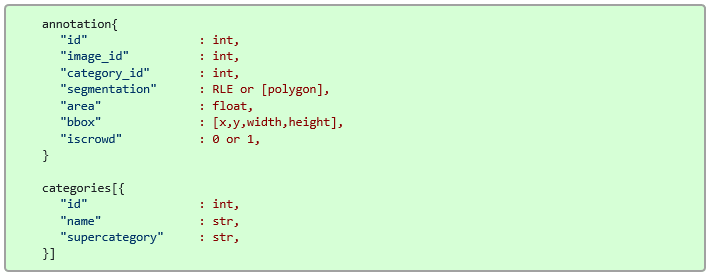
\includegraphics[width=11cm]{./Coco_Annotation_2}
\caption{Estructura básica de anotaciones en COCO.}
\label{AnnotacionesCoco2}
\end{center}
\end{figure}

En referencia a los datos, el conjunto de datos MS COCO se divide en dos partes aproximadamente iguales. La primera mitad del conjunto de datos se lanzó en 2014, mientras que la segunda mitad se lanzó en 2015. La versión 2014 contiene \textbf{82.783} imágenes para el entrenamiento, \textbf{40.504} para validaciones y \textbf{40.775} imágenes de prueba (aproximadamente 1/2 de imágenes de entrenamiento, 1/4 de validación y 1/4 de prueba). Hay casi 270 mil personas segmentadas y un total de 886 mil instancias de objetos segmentados en los datos de entrenamiento y validación. La versión acumulada de 2015 contendrá un total de \textbf{165.482} imágenes de entrenamiento, \textbf{81.208} de validación y \textbf{81.434} de prueba.\\

La distribución de los objetos en esta base de datos se puede obtener desde su sitio web. En la sección \textit{Explorar}, es posible elegir y combinar cada uno de los objetos y observar cuántas imágenes aparecen. La distribución de cada uno de los objetos en el conjunto de entrenamiento / validación se muestra en la siguiente imagen:

\begin{figure}[H]
\begin{center}
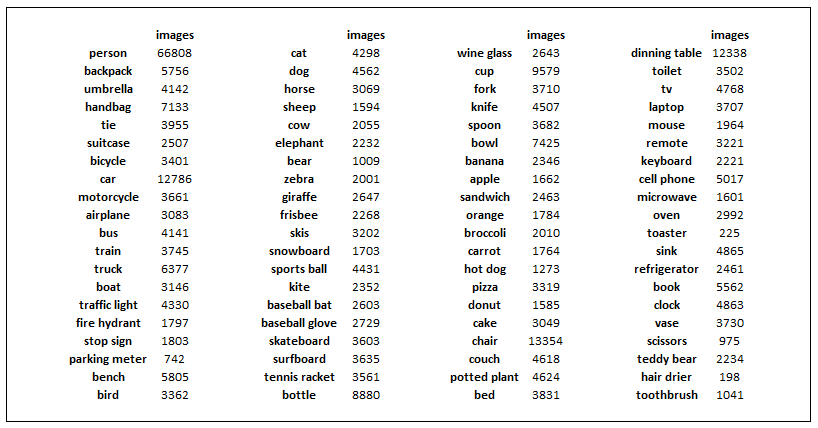
\includegraphics[width=13cm]{./COCO_Statics}
\caption{Distribución de objetos en COCO.}
\end{center}
\end{figure}

\chapter{Detección con Single Shot MultiBox y Caffe}
\markboth{DETECCIÓN}{DETECCION}

\section{Técnica Single Shot MultiBox Detection}
\lhead[\thepage]{\thesection. Técnica SSD}

Single Shot MultiBox Detector (SSD) es un framework diseñado para detectar objetos en imágenes utilizando para ello únicamente una red neuronal profunda. Fue lanzado a finales de noviembre de 2016 y obtuvo resultados muy positivos en términos de rendimiento y precisión en tareas de detección de objetos obteniendo más del 74\% en \textit{mAP} (mean Average Precision) a 59 \textit{frames} por segundo en conjuntos de datos estándar como PascalVOC y COCO. Para una mejor comprensión de esta técnica, se puede comenzar con definir el significado de su nombre:

\begin{itemize}
\item \textbf{Single Shot:}  Hace referencia a que la tareas de localización y clasificación de objetos se realizan en un único paso hacia adelante de la red.
\item \textbf{MultiBox:} Es el nombre de una técnica para regresión de \textit{bounding box} desarrollada por Szegedy.
\item \textbf{Detector:} La red neuronal se trata de un detector de objetos que también clasifica esos objetos detectados.
\end{itemize}

En el momento de la predicción, la red neuronal genera las puntuaciones para cada categoría de objetos en cada cuadro predeterminado y produce ajustes en este cuadro para ajustarse mejor a la forma del objeto. Además, la red combina predicciones de múltiples mapas de características con diferentes resoluciones para manejar de forma natural objetos de varios tamaños.

\begin{figure}[H]
\begin{center}
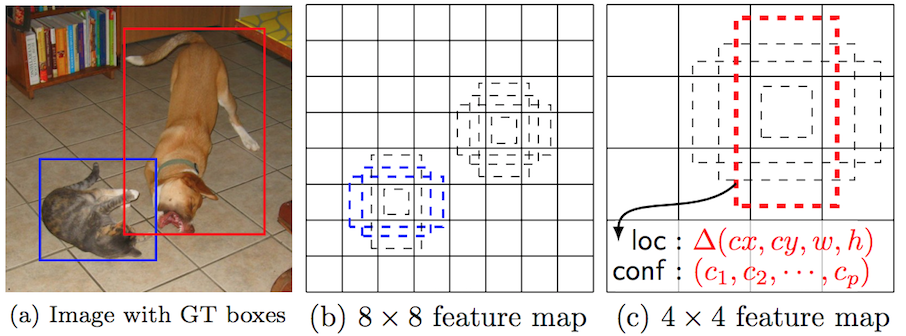
\includegraphics[width=13cm]{./FrameworkSSD}
\caption{Framework SSD. Imagen obtenida de \cite{SSD}.}
\label{FrameworkSSD}
\end{center}
\end{figure}

(a) SSD solo necesita una imagen de entrada y los cuadros delimitadores reales para cada objeto durante el entrenamiento. De una manera convolucional, se evalúa un pequeño conjunto de cuadros predeterminados (p.ej. 4) de diferentes relaciones de aspecto para cada ubicación de éstos en varios mapas de características a diferentes escalas (p. ej 8 x 8 y 4 x 4 en (b) y (c). Para cada cuadro predeterminado se predicen tanto los desplazamiento de forma como la confianza para todas las categorías de objetos (\textit{(c1, c2, ..., cp)}). En el momento del entrenamiento, se comparan estos cuadros predeterminados con los cuadros reales.

\subsection{Arquitectura}\label{ArquitecturaSSDSection}

El modelo SSD se basa en una red convolucional que produce un conjunto de recuadros delimitadores o \textit{bounding boxes} de tamaño fijo y puntuaciones para la presencia de instancias de clases de objetos dentro de esos cuadros, seguido por un paso de supresión no máxima para producir las detecciones finales. Las primeras capas de la red se basan en una arquitectura VGG-16 pero descartando las capas totalmente conectadas de ésta. La razón por la que se usa VGG-16 es su gran desempeño en la clasificación de imágenes de alta calidad. En lugar de las capas totalmente conectadas de VGG, se agregaron un conjunto de capas convolucionales auxiliares, lo que permite extraer características en múltiples escalas y disminuir progresivamente el tamaño de la imagen de entrada. Posteriormente, se agrega una estructura auxiliar a la red para producir detecciones. Esta estructura tiene las siguientes características claves:

\begin{itemize}
\item \textbf{Mapas de características con múltiples escalas para la detección:}  Se agregan varias capas de convolucionales al final de la estructura estándar comentada anteriormente. Estas capas disminuyen de forma progresiva el tamaño de la imagen de entrada y permiten predecir detecciones a múltiples escalas. 
\item \textbf{Predictores convolucionales para la detección:}  Cada capa de características añadida puede producir un conjunto fijo de predicciones de detección utilizando para ello un conjunto de filtros convolucionales. Estos filtros están indicados en la parte superior de la arquitectura de la red SSD en la figura \ref{ArquitecturaSSD}. Para una capa de características de tamaño \textit{m X n} con \textit{p} canales, el elemento básico para predecir los parámetros de una posible detección es un núcleo pequeño de 3 x 3 x \textit{p} el cuál produce una puntuación para una categoría determinada. En cada una de las posiciones por donde se aplica el filtro, éste produce un valor de salida.

\begin{figure}[H]
\begin{center}
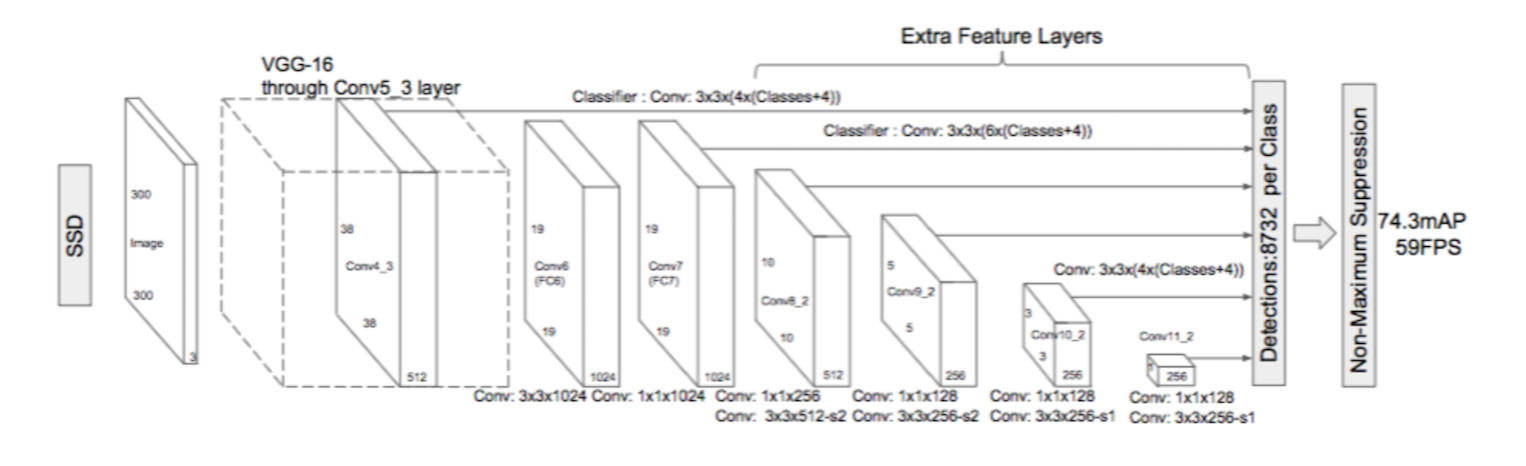
\includegraphics[width=15cm]{./SSD_Architecture}
\caption{Arquitectura SSD. Imagen obtenida de \cite{SSD}.}
\label{ArquitecturaSSD}
\end{center}
\end{figure}

\item \textbf{Cajas predeterminadas y relaciones de aspecto:} Se asocian un conjunto de cuadros delimitadores por defecto con cada celda del mapa de características. Los cuadros predeterminados marcan el mapa de características de un manera convolucional, por lo que la posición de cada cuadro con respecto a su celda es fija. En cada celda del mapa de características, se predicen los desplazamientos relativos a las formas de los cuadros predeterminados en cada una de las celdas, así como la puntuación por clase que indica la presencia de una instancia de clase en cada uno de los cuadros delimitadores. Específicamente, para cada cuadro \textit{k} en una posición determinada se calcula la puntuación de clase \textit{c} y los 4 desplazamientos relativos a la forma del cuadro por defecto original. Como resultado se obtienen \textit{(c + 4)k} filtros que se aplican alrededor de cada ubicación en el mapa de características, produciendo \textit{(c + 4)kmn} de salidas para un mapa de \textit{m} x \textit{n}. Se permiten diferentes formas para los cuadros predeterminados en los mapas de características con el objetivo de discretizar el espacio para las posibles formas que tengan las cuadros delimitadores de salida.
\end{itemize}

\begin{figure}[H]
\begin{center}
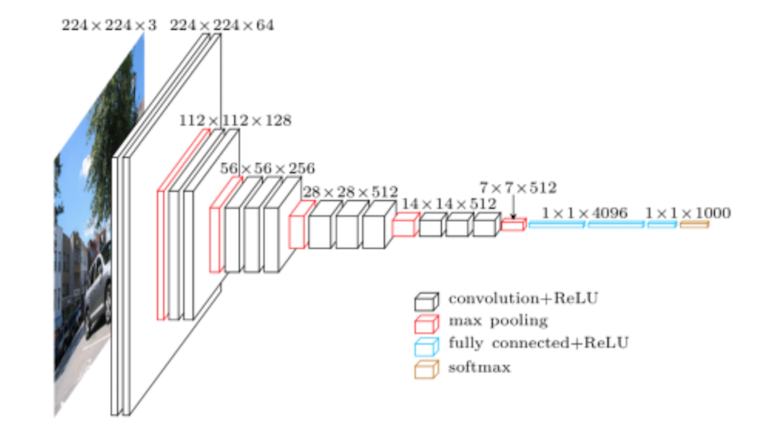
\includegraphics[width=13cm]{./VGG-16}
\caption{Arquitectura VGG-16. Imagen obtenida de \cite{SSD_2}.}
\label{VGG-16}
\end{center}
\end{figure}

\subsection{Entrenamiento}

La principal diferencia entre el entrenamiento usando la técnica SSD y el entrenamiento de un detector típico, es que la información a cerca de los cuadros delimitadores reales debe asignarse a salidas específicas dentro del conjunto fijo de salidas del detector. Tras realizar esta asignación, la función de pérdida y la propagación hacia atrás son aplicadas de extremo a extremo. El proceso de entrenamiento también implica elegir el conjunto de cuadros y escalas predeterminados para la detección.

\begin{itemize}
\item \textbf{Negativos:} Durante el entrenamiento, muchas de las \textit{bounding boxes} tienen un nivel muy bajo de \textit{IoU} y por lo tanto son interpretados como ejemplos de entrenamiento negativos. Esto provoca un significante desequilibrio entre ejemplos de entrenamiento positivos y negativos. En lugar de utilizar todos los ejemplos negativos, se ordenan usando la mayor pérdida de confianza para cada cuadro predeterminado y se seleccionan los más altos para asegurar que la relación de aspecto entre los negativos y los positivos sea como máximo 3:1. Esto provoca una optimización más rápida y un entrenamiento más estable.\\

\begin{figure}[H]
\begin{center}
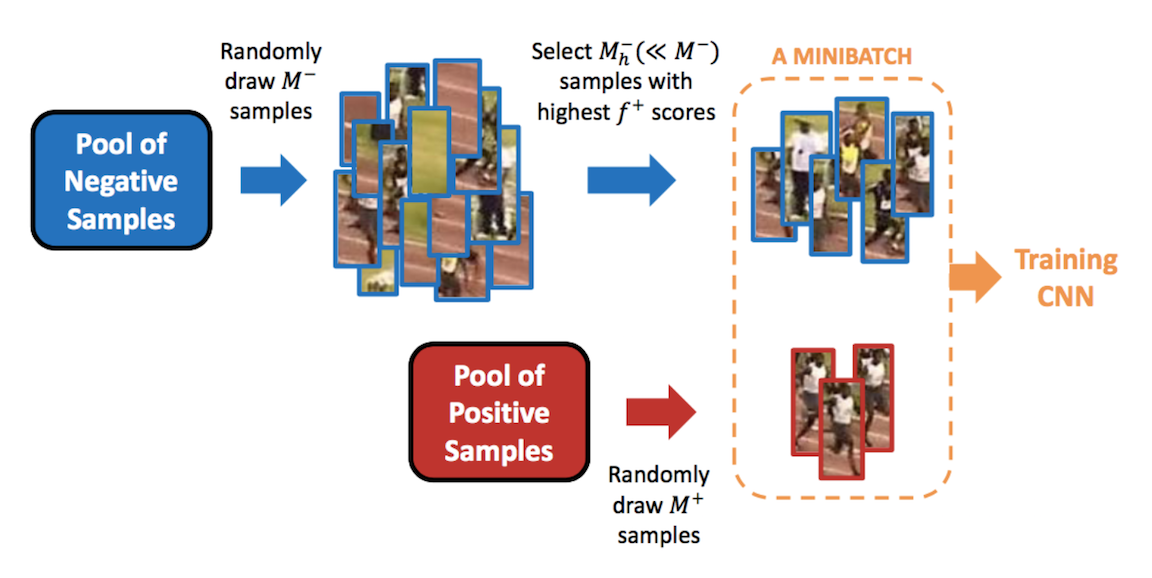
\includegraphics[width=13cm]{./HardNegativeMining}
\caption{Ejemplo de uso de negativos en el entrenamiento SSD. Imagen obtenida de \cite{SSD_2}.}
\label{VGG-16}
\end{center}
\end{figure}

\item \textbf{Aumento de datos:} El aumento de datos, tanto en la técnica SSD como en muchas otras aplicaciones de aprendizaje profundo, ha sido crucial para que la red neuronal sea mucho más robusta frente a diferentes tamaños y formas de objetos a la entrada de ésta. Con este fin, se generaron ejemplos de entrenamiento con parches de la imagen original con diferentes relaciones de IoU (p.ej. 0.1, 0.3, 0.5, etc). Además, cada imagen se gira horizontalmente de forma aleatoria con una probabilidad de 0.5, asegurando así que los objetos aparezcan con la misma probabilidad a la izquierda que a la derecha. 
\end{itemize}

\section{Single Shot MultiBox Detection en Caffe}\label{SSDCaffe}
\lhead[\thepage]{\thesection. SSD en Caffe}

Tras entender el funcionamiento de la técnica SSD, se realizará un ejemplo práctico que proporciona la herramienta Caffe. En este primer caso, se utilizarán algunos de los modelos preentrenados proporcionados en el repositorio oficial de los desarrolladores de la técnica SSD \cite{CaffeSSD}. Particularmente, se utilizarán 2 modelos, uno que utiliza la base de datos PascalVOC y otro que utiliza COCO, con el objetivo de realizar una primera y pequeña comparación entre la capacidad para detectar determinados objetos que tienen las redes entrenadas con ambas bases de datos.

\begin{itemize}
\item \textbf{PascalVOC07+12-SSD300x300:} Se trata de un modelo entrenado por el conjunto de las imágenes de entrenamiento de la base de datos PascalVOC de 2007 y 2012, con unas dimensiones de 300x300 píxeles.
\item \textbf{COCO-SSD300x300:} Se trata de un modelo entrenado utilizando la base de datos COCO. Se utiliza una dimensión de imagen de 300x300 píxeles.
\end{itemize}

Tras definir los modelos que se usarán, se crea el script \textit{image\_detection.py}, el cual, a partir de una imagen de entrada, realizará una serie de transformaciones sobre esta con el objetivo de adaptarla a la entrada de la red neuronal, la introducirá dentro de ésta y finalmente generará como salida esa misma imagen con las \textit{bounding boxes} sobre los objetos detectados. Este script será creado a partir del fichero \textit{ssd\_detect.ipynb}, desarrollado por los creadores de SSD y facilitado en su repositorio \cite{CaffeSSD}.\\

En primer lugar, se definen 3 ficheros que tendrán gran importancia a lo largo del proceso de detección:

\begin{itemize}
\item \textbf{labelmap.prototxt:} Define las etiquetas que pueden ser asignadas en la detección.
\item \textbf{model\_def:} Define la estructura básica de la red neuronal, la cual será explicada en el apartado \ref{Estructura}.
\item \textbf{model\_weights:} Se trata de un fichero binario que contiene el estado actual de los pesos para cada capa de la red neuronal.
\end{itemize}

Tras esto, utilizando la función de Caffe \textit{Net}, se define la red neuronal al completo, indicando tanto su estructura como los pesos de cada una de las capas, ambos datos almacenados en las variables \textit{model\_def} y \textit{model\_weights} comentadas anteriormente.\\

\begin{lstlisting}[frame=single]
self.net = caffe.Net(model_def,  # defines the structure of the model
				model_weights,  # contains the trained weights
				caffe.TEST)     # use test mode
\end{lstlisting}

Posteriormente, se define la función \textit{get\_labelname}, que es la encargada de devolver las etiquetas que se encuentran definidas en el fichero {labelmap.prototxt}.\\

\begin{lstlisting}[frame=single]
def get_labelname(self,labelmap, labels):
    num_labels = len(labelmap.item)
    labelnames = []
    if type(labels) is not list:
        labels = [labels]
    for label in labels:
        found = False
        for i in xrange(0, num_labels):
            if label == labelmap.item[i].label:
                found = True
                labelnames.append(labelmap.item[i].display_name)
                break
        assert found == True
    return labelnames
    
\end{lstlisting}

Finalmente, se define la función \textit{detection\_test}, la cual toma una imagen como entrada y retorna esta misma imagen con las bounding boxes de los objetos detectados superpuestas.

\begin{itemize}
\item Primero, esta función realiza una serie de transformaciones para adaptar la imagen de entrada a la red neuronal entrenada. Para ello, se utiliza la función \textit{Transformer} proporcionada por caffe. 
\item Después, la imagen transformada se introduce en la red usando el siguiente código.\\

\begin{lstlisting}[frame=single]
self.net.blobs['data'].data[...] = transformed_image
\end{lstlisting}

\item Después de esto, comienza la parte de la detección. Para ello, se utiliza la siguiente función de Caffe, la cual devuelve las detecciones obtenidas.\\

\begin{lstlisting}[frame=single]
detections = self.net.forward()['detection_out']
\end{lstlisting}

\item Esta salida es parseada en varios vectores que contienen las etiquetas de los objetos detectados, su confianza y las coordenadas de su \textit{bounding box}.\\

\begin{lstlisting}[frame=single]
det_label = detections[0,0,:,1] 
det_conf = detections[0,0,:,2] 
det_xmin = detections[0,0,:,3] 
det_ymin = detections[0,0,:,4] 
det_xmax = detections[0,0,:,5] 
det_ymax = detections[0,0,:,6]
\end{lstlisting}

\item Es importante no seleccionar todas las detecciones obtenidas, ya que algunas de ellas con un valor de confianza bajo pueden no ser tan precisas como se desee. Para ello, se usa un filtro que elige las detecciones con un nivel de confianza mayor a 0.6.\\

\begin{lstlisting}[frame=single]
# Get detections with confidence higher than 0.6. 
for i in range(0, len(det_conf)): 
    if (det_conf[i] >= 0.6): 
        top_indices.append(i) 

top_conf = det_conf[top_indices] 
top_label_indices = det_label[top_indices].tolist() 
top_labels = self.get_labelname(self.labelmap, 
						top_label_indices) 
top_xmin = det_xmin[top_indices] 
top_ymin = det_ymin[top_indices] 
top_xmax = det_xmax[top_indices] 
top_ymax = det_ymax[top_indices] 
\end{lstlisting}

\end{itemize}


\section{Detector de objetos}
\lhead[\thepage]{\thesection. Detector de objetos}

\subsection{Estructura de la red}\label{Estructura}

En esta sección se explicará la estructura de la red neuronal, la cual entrenaremos con las bases de datos definidas en los apartados \ref{VOC} y \ref{COCO} pare realizar posteriormente la detección de objetos sobre una imagen de entrada.\\

En primer lugar, se especificará el nombre de la red, en este caso \\'VGG\_VOC0712\_SSD\_300x300\_deploy'.\\

\begin{lstlisting}[frame=single]
name: "VGG_VOC0712_SSD_300x300_deploy"
\end{lstlisting}

Al inicio, también es necesario definir la dimensiones que tendrán las imágenes usadas para el entrenamiento. Tanto en PascalVOC como COCO, las imágenes tienen una dimensión de 300x300 y un formato RGB, definiéndose en la red de la siguiente manera:\\

\begin{lstlisting}[frame=single]
input_shape {
  dim: 1
  dim: 3
  dim: 300
  dim: 300
}
\end{lstlisting}

Como se ha explicado en la sección \ref{ArquitecturaSSDSection}, la arquitectura de la red neuronal en la técnica SSD se basa en las redes convolucionales, por lo que a continuación se pueden observar varias capas de convolución combinadas con capas de pooling.\\

En primer lugar, se define la capa de convolución, cuyo funcionamiento se ha explicado en la sección \ref{CapasVision}.\\

\begin{lstlisting}[frame=single]
layer {
  name: "conv1_1"
  type: "Convolution"
  bottom: "data"
  top: "conv1_1"
  param {
    lr_mult: 1.0
    decay_mult: 1.0
  }
  param {
    lr_mult: 2.0
    decay_mult: 0.0
  }
  convolution_param {
    num_output: 64
    pad: 1
    kernel_size: 3
    weight_filler {
      type: "xavier"
    }
    bias_filler {
      type: "constant"
      value: 0.0
    }
  }
}
\end{lstlisting}

Al inicio de esta capa se definen varios parámetros tales como el nombre de esta, \textit{name}, el tipo, \textit{type}, la capa de la cual recibe los datos, \textit{bottom} y la capa a la cual enviará los datos procesados, \textit{top}. Este ejemplo particular de capa de convolución generará 64 salidas, \textit{num\_output} y utilizará un núcleo de convolución de 3x3, \textit{kernel\_size}. Para inicializar los pesos se utilizará el algoritmo Xavier, el cual determina automáticamente la escala de inicialización basándose en el número de entradas y salidas de cada neurona. Adicionalmente, el sesgo se inicializará como una constante, siendo esta 0.0.\\

Posteriormente se define una capa de pooling, cuyo funcionamiento se ha explicado en el apartado \ref{CapasVision}.\\

\begin{lstlisting}[frame=single]
layer {
  name: "pool1"
  type: "Pooling"
  bottom: "conv1_2"
  top: "pool1"
  pooling_param {
    pool: MAX
    kernel_size: 2
    stride: 2
  }
}
\end{lstlisting}

Esta capa tomará los datos de la capa de convolución anterior y utilizará bloques de 2x2 para dividir la imagen entrante. Para que no haya solapamiento entre bloques contiguos utilizará el parámetro \textit{stride = 2}. Finalmente, como función de agrupación utilizará el máximo, escogiendo el píxel con mayor nivel de intensidad de cada bloque.\\

Entre las capas da convolución y pooling, se intercalan varias capas de activación, utilizando la función ReLU, explicada en el apartado \ref{CapasActivacion}.\\

\begin{lstlisting}[frame=single]
layer {
  name: "relu1_1"
  type: "ReLU"
  bottom: "conv1_1"
  top: "conv1_1"
}
\end{lstlisting}

En esta capa simplemente se definirán los parámetros comunes que se definen en todas las capas de la red, es decir, nombre de ésta, tipo, capa de la que recibe los datos y capa a la cual se los enviará.\\

Además de las capas de activación, existirán varias capas de diferentes tipos que procesarán los datos obtenidos de diferentes maneras.

\begin{itemize}
\item Las capas de datos de tipo \textit{Flatten} transforma una entrada de dimensiones \textit{n * c * h * w} en un vector simple de dimensiones \textit{n * (c*h*w)}\\
\begin{lstlisting}[frame=single]
layer {
  name: "conv4_3_norm_mbox_loc_flat"
  type: "Flatten"
  bottom: "conv4_3_norm_mbox_loc_perm"
  top: "conv4_3_norm_mbox_loc_flat"
  flatten_param {
    axis: 1
  }
}
\end{lstlisting}
\item Las capas de datos de tipo \textit{Reshape} recibe como entrada una capa de unas dimensiones arbitrarias y genera como salida las misma capa pero con las dimensiones definidas en \textit{reshape\_param}.\\
\begin{lstlisting}[frame=single]
layer {
  name: "mbox_conf_reshape"
  type: "Reshape"
  bottom: "mbox_conf"
  top: "mbox_conf_reshape"
  reshape_param {
    shape {
      dim: 0
      dim: -1
      dim: 21
    }
  }
}
\end{lstlisting}

Las dimensiones de salida están especificadas en \textit{reshape\_param}. Los números positivos se utilizan directamente, configurando la dimensión correspondiente en la capa de salida. Además, se aceptan 2 valores especiales para definir cualquier que se desee.
\begin{itemize}
\item Si se utiliza el valor \textbf{0} se copiará la dimensión de la capa inferior, es decir, si la capa inferior tiene 2 como su primera dimensión, la capa superior tendrá 2 como su primera dimensión.
\item Si se utiliza \textbf{-1} se reducirá este valor de las otras dimensiones.
\end{itemize}
\item Las capas de datos de tipo \textit{Concat} concatena varias capas de entrada en una única capa de salida.\\
\begin{lstlisting}[frame=single]
layer {
  name: "mbox_loc"
  type: "Concat"
  bottom: "conv4_3_norm_mbox_loc_flat"
  bottom: "fc7_mbox_loc_flat"
  bottom: "conv6_2_mbox_loc_flat"
  bottom: "conv7_2_mbox_loc_flat"
  bottom: "conv8_2_mbox_loc_flat"
  bottom: "conv9_2_mbox_loc_flat"
  top: "mbox_loc"
  concat_param {
    axis: 1
  }
}
\end{lstlisting}
Suponiendo que se recibe una entrada \textit{n\_i * c\_i * h * w} para cada capa de entrada \textit{it}.
\begin{itemize}
\item Si \textit{axis = 0}, \textit{(n\_1 + n\_2 + ... + n\_K) * c\_1 * h * w} y todas las entrada \textit{c\_i} deberían ser iguales.
\item Si \textit{axis = 1}, \textit{(n\_1 * (c\_1 + c\_2 + ... + c\_K) * h * w} y todas las entrada \textit{n\_i} deberían ser iguales.
\end{itemize}
\end{itemize}

Finalmente, se define la capa que determina la salida.\\

\begin{lstlisting}[frame=single]
layer {
  name: "detection_out"
  type: "DetectionOutput"
  bottom: "mbox_loc"
  bottom: "mbox_conf_flatten"
  bottom: "mbox_priorbox"
  top: "detection_out"
  include {
    phase: TEST
  }
  detection_output_param {
    num_classes: 21
    share_location: true
    background_label_id: 0
    nms_param {
      nms_threshold: 0.449999988079
      top_k: 400
    }
    save_output_param {
      output_directory: "/home/davidbutra/data/VOCdevkit/
      				results/VOC2007/SSD_300x300/Main"
      output_name_prefix: "comp4_det_test_"
      output_format: "VOC"
      label_map_file: "data/VOC0712/labelmap_voc.prototxt"
      name_size_file: "data/VOC0712/test_name_size.txt"
      num_test_image: 4952
    }
    code_type: CENTER_SIZE
    keep_top_k: 200
    confidence_threshold: 0.00999999977648
  }
}
\end{lstlisting}

\subsection{Definición del solucionador}

El solucionador es el responsable de la optimización del modelo y se define en un archivo con extensión \textit{.prototxt}. Aquí, se especifican los parámetros necesarios para ejecutar de forma correcta el entrenamiento. Más concretamente, el solucionador se encarga de:

\begin{itemize}
\item Crea la red de entrenamiento para el aprendizaje y la red de test para la evaluación.
\item Optimiza de forma iterativa realizando llamadas hacia delante y hacia atrás de la red, actualizando al mismo tiempo los parámetros de esta.
\item Periódicamente, evalúa las redes de prueba.
\item Crea instantáneas del modelo y del estado del solucionador a lo largo de la optimización.
\end{itemize}

En cada iteración, el solucionador realiza las siguientes operaciones:

\begin{itemize}
\item Cálculo de la salida de la red y de la pérdida.
\item Llamada hacia atrás a la red para calcular el gradiente.
\item Incorpora los gradientes en las actualizaciones de los parámetros según el método del solucionador.
\item Actualiza el estado del solucionador de acuerdo con la velocidad de aprendizaje, el historial y el método.
\end{itemize}

A continuación, se muestra el aspecto del solucionador usado para el entrenamiento de la red, llamado \textit{solver.prototxt}:\\

\begin{lstlisting}[frame=single]
train_net: "models/VGGNet/VOC0712/SSD_300x300/train.prototxt"
test_net: "models/VGGNet/VOC0712/SSD_300x300/test.prototxt"
test_iter: 619
test_interval: 10000
base_lr: 0.001
display: 10
max_iter: 120000
lr_policy: "multistep"
gamma: 0.1
momentum: 0.9
weight_decay: 0.0005
snapshot: 80000
snapshot_prefix: "models/VGGNet/VOC0712/SSD_300x300/VGG_VOC0712_SSD_300x300"
solver_mode: GPU
device_id: 0
debug_info: false
snapshot_after_train: true
test_initialization: false
average_loss: 10
stepvalue: 80000
stepvalue: 100000
stepvalue: 120000
iter_size: 1
type: "SGD"
eval_type: "detection"
ap_version: "11point"
\end{lstlisting}

Uno de los primeros parámetros que hay que especificar es \textit{type}, el cual determina el tipo de solucionador que se va a utilizar. En Caffe existen 6 tipos diferentes de solucionadores, cuyas características y funcionalidades se pueden consultar en la documentación oficial de Caffe\footnote{\url{http://caffe.berkeleyvision.org/tutorial/solver.html}}. Para este caso en particular, se ha utilizado el tipo \textit{SGD, Stochastic Gradient Descent}.\\

Otros de los parámetros que se pueden destacar dentro este fichero son, \textit{train\_net} y \textit{test\_net} que muestran la localización de los ficheros que especifican la estructura de la red; \textit{solver\_mode}, que específica si se va a utilizar la unidad central o la unidad gráfica de procesamiento, en este caso será CPU; \textit{base_lr}, que fija el ritmo de aprendizaje, \textit{learning rate}, durante el entrenamiento; \textit{lr_policy} que determina la política que seguirá la ritmo de aprendizaje, en este caso será \textit{step}, que indica que cada cierto tiempo se reducirá la tasa de aprendizaje; \textit{gamma} que especifica cuanto se va a reducir el \textit{learning rate} cada \textit{step}; \textit{stepsize} que determina cada cuantas iteraciones o \textit{steps} se reducirá el ritmo de aprendizaje; \textit{max\_iter}, que define el número máximo de iteraciones que se van a realizar en el entrenamiento;

\subsection{Entrenamiento de la red}

Antes de comenzar el entrenamiento de la red neuronal, es necesario definir las imágenes con las que vamos a alimentar a ésta durante el el proceso. Pare este caso, se decidió crear una base de datos personalizada la cuál contendrá tanto las imágenes de entrenamiento de PascalVoc de los años 2007 y 2012 como las de COCO. Para componerla, es necesario obtener los ficheros \textit{.lmdb} que incluyen toda la información de ambas bases de datos. Para ello, se dispone de los siguientes recursos y documentación:

\begin{itemize}
\item En el repositorio \textit{GIT} de los desarrolladores de la técnica SSD\footnote{\url{https://github.com/weiliu89/caffe/tree/ssd}}, en el apartado \textbf{Preparation}, se explica paso a paso todo el proceso para crear los ficheros LMDB que contendrán las imágenes y anotaciones de la base de datos PascalVoc.
\item En el repositorio \textit{GIT} referenciado\footnote{\url{https://github.com/intel/caffe/tree/master/data/coco}} se explica como crear los ficheros LMDB que contendrán la información de la base de datos COCO.
\end{itemize}

Tras esto, se creó el \textit{script create_lmdb.py}\footnote{\url{https://github.com/RoboticsURJC-students/2016-tfg-David-Butragueno/blob/master/create_lmdb.py}} que será el encargado de fusionar en un único fichero LMDB toda la información de ambas bases de datos existente en los archivos creados anteriormente.\\

Para el entrenamiento de la red neuronal, los desarrolladores de SSD generaron varios \textit{scripts} que cumplen este objetivo. Particularmente, se destacan los \textit{scripts} \textit{ssd\_pascal.py} y \textit{ssd\_coco.py}, facilitados en el repositorio oficial de los creadores de esta técnica, y cuya finalidad es el entrenamiento de la red utilizando las imágenes de entrenamiento y validación de las bases de datos PascalVoc y COCO respectivamente. En estos \textit{scripts} se encuentran tanto las rutas de todos los ficheros necesarios para el entrenamiento, ya sea el modelo, el mapa de etiquetas, el solucionador o los archivos que alimentaran a la red de imágenes durante el proceso, como las rutas dónde se almacenaran los resultados del entrenamiento. Finalmente, a partir de los datos provistos, se crean la red neuronal y el solucionador, necesarios para lanzar el entrenamiento.\\

Por lo tanto, para este caso, se creo un \textit{script} adicional, a partir de los mencionados anteriormente, modificando todos los datos necesarios.Tras la ejecución de este \textit{script}, comienza el entrenamiento, mostrando por la pantalla del terminal información del propio proceso cada 10 iteraciones.\\

\begin{figure}[H]
\begin{center}
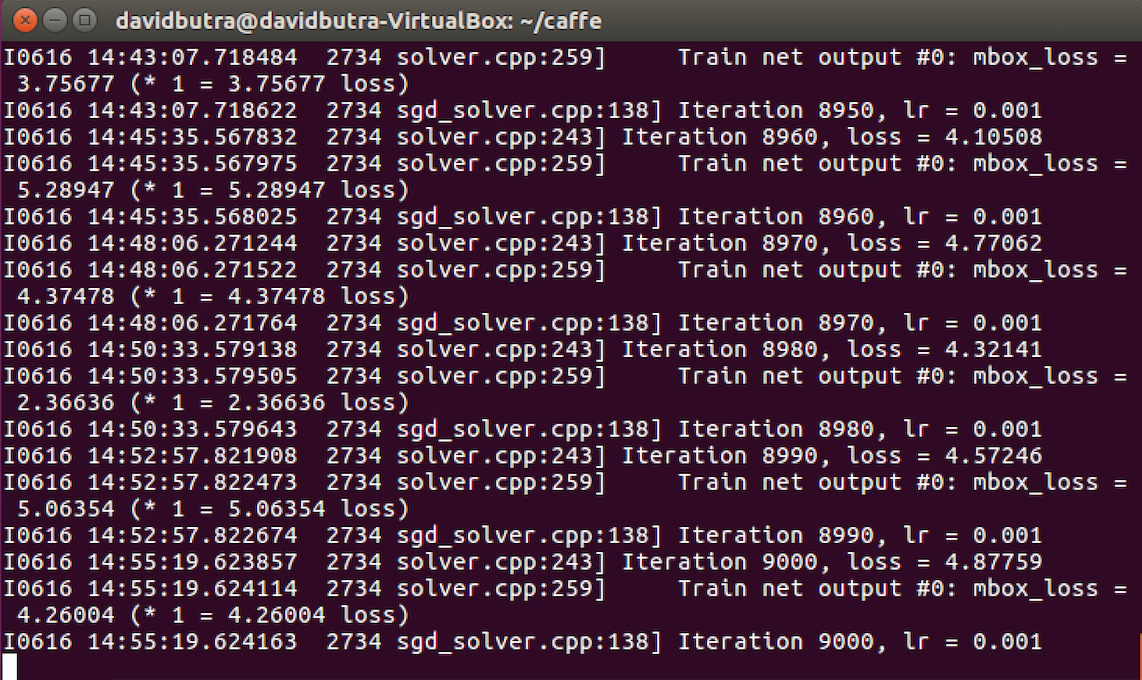
\includegraphics[width=13cm]{./TrainNet}
\caption{Ejecución de entrenamiento de la red neuronal.}
\label{EjecucionTrain}
\end{center}
\end{figure}

Durante la ejecución, cada 1000 iteraciones, se genera una \textit{snapshot} en forma de fichero binario con extensión \textit{.caffemodel} que contiene los pesos existentes en cada una de las capas de la red neuronal en ese momento del entrenamiento.

\section{Componente 
 detector}
\lhead[\thepage]{\thesection. Componente JdeRobot detector}\label{ComponenteDetector}

Con el objetivo de entender mejor todo lo comentado anteriormente, se desarrolla un componente en Python que, a partir del \textit{Camera Server} de JdeRobot explicado en el apartado \ref{Camera}, será capaz de realizar la detección en tiempo real de las imágenes captadas por la cámara. La imagen \ref{ComponenteDetector} muestra un diagrama de bloques con el diseño de este componente.\\

Para mejorar el rendimiento de este componente, se ha desacoplado en 3 hilos de ejecución que serán explicados a continuación:

\begin{itemize}
\item \textit{Hilo Camera:} Será el encargado de capturar las imágenes captadas por la cámara utilizando para ello el servidor de imágenes, \textit{Camera Server}. Esta imagen será enviada al \textit{hilo GUI} para su visualización y al \textit{hilo Detector} para su procesamiento. 
\item  \textit{Hilo Detector:} Este hilo será el encargado de la detección. Para ello, realiza las transformaciones que sean necesarias de la imagen que recibe desde el \textit{hilo Camera}, y, como se ha explicado en el apartado \ref{SSDCaffe}, realiza la detección de ésta. Tras generar como salida la misma imagen con las \textit{bounding boxes} de los objetos detectados superpuestas, la envía al \textit{hilo GUI} para su visualización.
\item \textit{Hilo GUI:} Será el encargado del aspecto gráfico de la aplicación, mostrando tanto la imagen real captada por la cámara como la imagen tras su procesamiento y la detección de objetos.
\end{itemize}

\begin{figure}[H]
\begin{center}
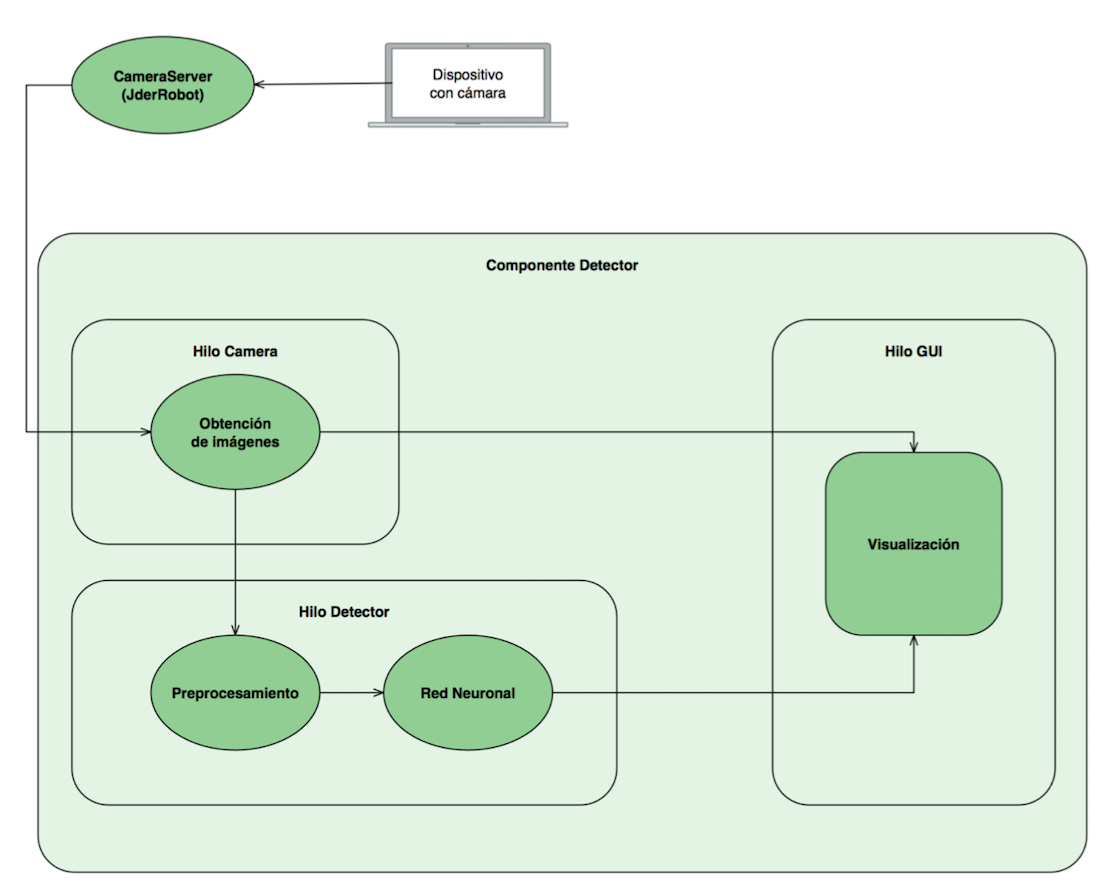
\includegraphics[width=13cm]{./ComponenteDetector}
\caption{Esquema del Componente Detector.}
\label{ComponenteDetector}
\end{center}
\end{figure}

\subsection{Hilo Camera}

Este hilo será el encargado de obtener la imagen capturada por la cámara, la cual será visualizada en el hilo encargado de la parte gráfica. Este hilo podrá ser referencia con el nombre de la clase, \textit{Camera()}.\\

Al inicializar esta clase, en el constructor, se especifica que se va a realizar una referencia externa, en forma de fichero de configuración. De esta manera, el hilo \textit{Camera()} se podrá conectar con el componente JdeRobot \textit{Camera Server}, y de así adquirir la imágenes que éste provee. El fichero de configuración, que se especifica en línea de comandos cuando se ejecuta el componente, se muestra a continuación.\\

\begin{lstlisting}[frame=single]
DetectorSSD.Camera.Proxy=cameraA:default -h localhost -p 9999
\end{lstlisting}

Tras el constructor de la clase y una vez que la aplicación está conectada con el componente JdeRobot, se definen 2 funciones de gran importancia para la ejecución de ésta. En primer lugar, se especifica el método \textit{getImage(self)} cuya función será obtener las imágenes de la cámara. También realiza una sería de transformaciones de éstas antes de que el \textit{hilo Detector} las introduzca en la red neuronal. Por último, se define la función \textit{update(self)} cuyo objetivo será actualizar la ejecución de este hilo. Este método será llamado desde la clase \textit{ThreadCamera} en la que se define que el ciclo de ejecución de este hilo será de 1500 milisegundos.

\subsection{Hilo Detector}

Este hilo será el encargado de todo el proceso de detección, desde el procesamiento de la imagen que recibe desde el \textit{hilo Camera} para adaptarla a lo que requiere la red neuronal, hasta la obtención de la salida de la red y la posterior generación de la imagen con las detecciones producidas.\\

Para realizar la detección, este hilo utilizará el mismo proceso explicado en el apartado \ref{SSDCaffe}, en el cual, a partir de una única imagen de entrada se genera como salida la misma imagen con las \textit{bounding boxes} de los objetos detectados superpuestos sobre ella. Así, en el constructor de este hilo se definirán las variables que hacen referencia al mapa de etiquetas que pueden ser asignadas en la detección, a la estructura de la red y a los pesos de la red entrenada. Tras esto, se define la función \textit{detectiontest(self,img)}, explicada en el apartado \ref{SSDCaffe} y que se encarga de introducir la imagen de entrada en la red neuronal y obtener las detecciones.\\

Finalmente, como en el \textit{hilo Camera}, se define la función \textit{update(self)} que actualizará la ejecución de este hilo. El ciclo de ejecución está especificado en la clase \textit{ThreadDetector} y será de 1500 milisegundos.

\subsection{Hilo GUI}

Este hilo será el encargado de todo el aspecto gráfico de la aplicación. Renderizará las 2 imágenes generadas en el resto de hilos, es decir, la capturada en tiempo real por el \textit{hilo Camera} y la imagen procesada en la que se muestra los objetos detectados recibida desde el \textit{hilo Detector}.\\

En el constructor de esta clase, en primer lugar se inicializará la ventana principal, en la que aparecerán todos los elementos comentados anteriormente.\\

\begin{lstlisting}[frame=single]
QtGui.QWidget.__init__(self, parent)
self.setWindowTitle("Detection Component")
self.resize(1200,500)
self.move(150,50)
self.updGUI.connect(self.update)
\end{lstlisting}

En el código anterior, se define el título que aparecerá en la parte superior de la ventana, \textit{setWindowTitle}, la anchura y altura de ésta, \textit{resize} y su posición, \textit{move}. Con la función \textit{connect} se le asocia la función \textit{update}, que se encargará de actualizar este hilo de ejecución.\\

Posteriormente, se definen las ventanas donde se visualizarán las 2 imágenes comentadas anteriormente. Éstas vienen parametrizadas igualmente por los parámetros \textit{resize} y \textit{move}.\\

Finalmente, se crean 2 botones, los cuales serán los encargados de controlar el proceso de detección. Estos botones, además de venir definidos por del parámetro \textit{move} para determinar su posición, se les añadirá la función \textit{setStyleSheet} con el objetivo de asociarles un color. Adicionalmente, utilizando \textit{clicked.connect} se les asignará la función que se ejecutará cuando se haga \textit{click} sobre cada uno de los 2 botones.\\

Tras el constructor de la clase GUI, se definirá la función \textit{update(self)} que actualizará la ejecución de este hilo. Aquí, se asignarán a cada una de las ventanas creadas la imagen captada de la cámara y la imagen con las detecciones obtenidas según corresponda.\\

Finalmente, se definirán las 2 funciones asociadas a los 2 botones creados anteriormente. La función \textit{toggle(self)} estará asociada al botón \textit{Continuos} y hará que tras pulsarlo, comience la detección continua de las imágenes captadas en tiempo real. Por otro lado, la función \textit{detectOnce(self)} estará asociada al botón \textit{Detect Once} y hará que al hacer \textit{click} sobre él, se realice la detección únicamente sobre el frame que se estaba mostrando por la cámara en ese momento exacto.

\subsection{Ejecución}

El proceso de ejecución de este componente estará divido en 2 pasos. Uno será el encargado de lanzar el servidor de imágenes, utilizando para ello el componente \textit{Camera Server} de JdeRobot. El otro será el encargado de lanzar el propio componente detector explicado en las secciones anteriores.\\

Para lanzar el componente \textit{Camera Server}, será necesario abrir un terminal y ejecutar el siguiente comando proporcionado por la plataforma JdeRobot.\\

\begin{lstlisting}[frame=single]
cameraserver cameraserver.cfg
\end{lstlisting}

Una vez que está lanzado el servidor de imágenes, se ejecutará el siguiente comando, el cual lanzará el propio componente detector.\\

\begin{lstlisting}[frame=single]
python detectorSSD.py --Ice.Config=detectorSSD.cfg
\end{lstlisting}

En primer lugar se hará referencia al script principal del componente, \textit{detectorSSD.py}, cuyo objetivo es lanzar los 3 hilos que lo forman. Posteriormente se especifica el fichero de configuración \textit{detectorSSD.cfg} gracias al cual se tendrá comunicación con el servidor de imágenes. Este fichero tiene una propiedad en la que se define el nombre de la cámara, el cual tiene que ser el mismo que el definido anteriormente en el fichero \textit{cameraserver.cfg} para que dicha conexión sea efectiva.\\

Finalmente, tras lanzar ambos comandos, se obtiene el componente detector explicado. A continuación se muestran 2 imágenes donde se aprecia el funcionamiento del componente. La imagen \ref{DeteccionContinua} se puede observar como se comporta la aplicación cuando se pulsa el botón encargado de realizar la detección continua. Por otro lado, la imagen \ref{DeteccionUnica} muestra el funcionamiento del componente tras pulsar el botón encargado de la detección única.

\chapter{Medidor de calidad}
\markboth{MEDIDOR DE CALIDAD}{MEDIDOR DE CALIDAD}

\section{Comparación \textit{bounding boxes} real y detectada}
\lhead[\thepage]{\thesection. Comparación \textit{BBs} real y detectada}

En el apartado \ref{SSDCaffe} se ha explicado como se obtiene la \textit{bounding box} de los objetos detectados. Para obtener la \textit{bounding box} real, hay que recuperar las coordenadas del objeto, las cuales se encuentran en las anotaciones de la imagen. Como se ha explicado en el apartado \ref{BBDD}, las anotaciones para PascalVOC y COCO tienen formatos de archivos diferentes, para la primera base de datos se trata de ficheros XML y para la segunda ficheros JSON, por lo que se utilizarán 2 scripts diferentes para recorrer el fichero determinado y obtener las coordenadas originales. Tras ello, se podrá observar fácil y gráficamente la diferencia entre la \textit{bounding box} real y la detectada, consiguiendo así una aproximación visual de la calidad del detector.

\subsection{PascalVOC}\label{ComparePascalVOC}

Se define la función \textit{get\_ground\_truth}, la cual devolverá un array por cada objeto detectado en el que vendrán informados las coordenadas de la \textit{bounding box} real, y la etiqueta del objeto determinado. Esta función recibirá como datos de entrada la ruta de la imagen de entrada, un array con las etiquetas de los objetos detectados y las coordenadas de las \textit{bounding boxes} de éstos.\\

En primer lugar, se utilizará la ruta de la imagen de entrada recibida (p.ej '/home/db/data/VOCdevkit/VOC2012/JPEGImages/2007\_009938.jpg') para obtener la ruta del fichero con las anotaciones correspondientes a esa imagen. Para ello, se utilizará el siguiente código:\\

\begin{lstlisting}[frame=single]
annotation = input_image.split(".")

annotation = annotation[0].split("/")

file_annotations = "/" + annotation[1] + "/" +  annotation[2] 
+ "/" + annotation[3] + "/" + annotation[4] + "/" + annotation[5] 
+"/" + 'Annotations' + "/" + annotation[7] + ".xml"
\end{lstlisting}

Realizando los 2 \textit{split} tendremos todas las partes de la ruta separadas dentro de la variable \textit{annotation}. Posteriormente, concatenando cada parte de la ruta con "/", sustituyendo \textit{JPEGImages} por \textit{Annotations}, e incluyendo el formato de los ficheros de anotaciones, es decir, \textit{xml}, tendremos la ruta del fichero de anotaciones correspondiente a la imagen de entrada.\\

Posteriormente, se utilizarán comandos \textit{Python} creados para la lectura de ficheros \textit{XML}, específicamente \textit{parse} y \textit{getroot}.\\

\begin{lstlisting}[frame=single]
tree = ET.parse(file)
root = tree.getroot()
\end{lstlisting}

A partir de este código, tendremos acceso a los elementos del fichero de anotaciones utilizando para ello la variable \textit{root}.\\

Después de esto, comenzará el primer bucle de esta función. Éste será el encargado de guardar en una variable varios datos de cada uno de los objetos existentes en el fichero de anotaciones. En primer lugar, el bucle buscará y recorrerá todas las etiquetas \textit{object} del \textit{xml}. Para ello se utilizará el comando de Python \textit{findall} sobre la variable \textit{root} definida anteriormente.\\

\begin{lstlisting}[frame=single]
for element in root.findall('object'):
\end{lstlisting}

Luego, con el comando \textit{find}, accederemos a las etiquetas \textit{name} y \textit{bbox} del fichero de anotaciones, guardando su valor en el array \textit{names\_xml} definido previamente.\\

\begin{lstlisting}[frame=single]
name = element.find('name').text
names_xml.append(name)
bndbox = element.find('bndbox')
names_xml.append(bndbox[0].text) #xmin
names_xml.append(bndbox[1].text) #ymin
names_xml.append(bndbox[2].text) #xmax
names_xml.append(bndbox[3].text) #ymax
\end{lstlisting}

Para mejorar el acceso posterior a estos datos, éstos se guardarán en un array de arrays, en el que cada array interno tendrá los datos mencionados anteriormente. Para ello, se definirá el array \textit{names\_xml\_final} y se guardará el array \textit{names\_xml} dentro de éste. Posteriormente, se eliminarán los datos guardados en el array \textit{names\_xml}.

\begin{lstlisting}[frame=single]
names_xml_final.append(names_xml)
names_xml = []
\end{lstlisting}

Tras finalizar este bucle, comenzará el código en el que se comparan las \textit{bounding boxes} reales con las detectadas para averiguar cuál es el cuadro delimitador real correspondiente para cada uno de los objetos detectados. En primer lugar se definirá un bucle, que recorrerá el array con todas las etiquetas de los objetos detectados el cual se pasó como parámetro a la función.\\

\begin{lstlisting}[frame=single]
for x in range(len(label_detection)):
\end{lstlisting}

Después, se definirán 2 bucles más. El primero recorrerá el array con las  coordenadas de los objetos detectados pasada a la función como parámetros. El segundo recorrerá el array \textit{names\_xml\_final} definido anteriormente.\\

\begin{lstlisting}[frame=single]
for t in range(len(ground_detection)):
	for i in range(len(names_xml_final)):
\end{lstlisting}

Ahora, el código comparará las coordenadas reales con las detectadas. Específicamente, se verificará que cada coordenada \textit{xmin}, \textit{ymin}, \textit{ymax}, \textit{ymax} de cada \textit{bounding box} de los objetos detectados no exceda en 40 píxeles con las coordenadas originales.\\

\begin{lstlisting}[frame=single]
if abs(int(ground_detection[t][0])-int(names_xml_final[i][1]))<=40
and abs(int(ground_detection[t][1])-int(names_xml_final[i][2]))<=40
and abs(int(ground_detection[t][2])-int(names_xml_final[i][3]))<=40
and abs(int(ground_detection[t][3])-int(names_xml_final[i][4]))<=40:
\end{lstlisting}

Con esto se conseguirá que cada \textit{bounding box} detectada se asigne correctamente a la \textit{bounding box} real, ya que si en el fichero de anotaciones existen varios objetos con la misma etiquetas, se podrían realizar asignaciones incorrectas si solo se compara la etiqueta y se obvian las coordenadas.\\

Posteriormente, tras verificar que las coordenadas son las correctas, se realizará la última comprobación. Ésta estará relacionada con la etiquetas de los objetos reales, almacenadas en la variable \textit{names\_xml\_final}, y las etiquetas de los objetos detectados, almacenadas en la variable \textit{label\_detection}, la cual fue pasada como parámetro a la función.\\

\begin{lstlisting}[frame=single]
if names_xml_final[i][0] == label_detection[x]
\end{lstlisting}

Tras esto, si se cumplen las condiciones, se asignarán a diferentes variables las coordenadas existentes en el fichero de anotaciones, es decir, las reales.\\

\begin{lstlisting}[frame=single]
xmin = names_xml_final[i][1]
ymin = names_xml_final[i][2]
xmax = names_xml_final[i][3]
ymax = names_xml_final[i][4]
\end{lstlisting}

Finalmente, la función devolverá el array \textit{positions\_array}, el cuán contendrá todas las variables comentadas anteriormente.\\

\begin{lstlisting}[frame=single]
positions = []
positions.append(xmin)
positions.append(ymin)
positions.append(xmax)
positions.append(ymax)
positions_array.append(positions)
\end{lstlisting}

Finalmente, las \textit{bounding boxes} reales se pintarán sobre la imagen de entrada a partir del array devuelto en la función anterior utilizando el siguiente código:\\

\begin{lstlisting}[frame=single]
for i in range(len(ground_truth)):
	xmin = int(round(float(ground_truth[i][0])))
	ymin = int(round(float(ground_truth[i][1])))
	xmax = int(round(float(ground_truth[i][2])))
	ymax = int(round(float(ground_truth[i][3])))

	cv2.rectangle(img,(xmin,ymin),(xmax,ymax),(0,255,0),2)#Color BGR
\end{lstlisting}

La imagen \ref{DetectionCompare} muestra un ejemplo de una salida que generaría este \textit{script}. La \textit{bounding box} de color verde hace referencia a las coordenadas reales del objeto, mientras que la \textit{bounding box} de color rojo encuadra el objeto detectado.\\

\begin{figure}[H]
\begin{center}
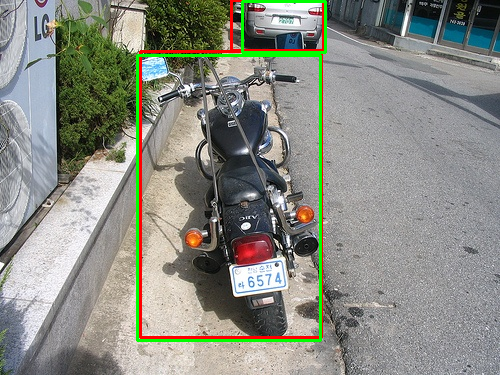
\includegraphics[width=11cm]{./image_detection_compare}
\caption{Comparacion bounding boxes real y detectada con imagen de la BBDD PascalVOC.}
\label{DetectionCompare}
\end{center}
\end{figure}

\subsection{COCO}\label{CompareCOCO}

Como se ha explicado en la sección \ref{COCO}, las anotaciones de esta base de datos están almacenadas en archivos de formato JSON, por lo que para conseguir las coordenadas reales de los objetos habrá que utilizar comandos que permitan recorrer este tipo de ficheros. Antes de realizar la función principal que devuelva la imagen con las \textit{bounding boxes} real y detectada superpuestas, se crearán varios métodos que recorrerán el fichero de anotaciones, preparando así los datos para ser tratados posteriormente.\\

En primer lugar, se definirá la función \textit{get\_image\_id}, la cual se encargará de obtener el \textit{id} de la imagen de entrada, que será necesario para encontrar las anotaciones correspondientes a ésta. Este \textit{id} se puede conseguir a partir del \textit{path} de la imagen \textit{jpg}, el cual se pasa como parámetro de la función.\\

\begin{lstlisting}[frame=single]
def get_image_id(self, image_file):

        image_file = re.split('.jpg', image_file)
        image_file = re.split('_', image_file[0])
        image_id = int(image_file[2])

        return image_id
\end{lstlisting}

La segunda función para la preparación de los datos se llamará \textit{annotations} y se encargará se recuperar todas las anotaciones de la imagen de entrada. Para ello se le pasará como parámetro el \textit{id} de la imagen calculado en la función explicada anteriormente.\\

Primero, se guardará en la variable \textit{jsonFileAnnotations} los objetos con nombre \textit{annotations} de todo el fichero de anotaciones \textit{jsonFile}, definido como variable global del script.\\

\begin{lstlisting}[frame=single]
jsonFileAnnotations = jsonFile["annotations"]
\end{lstlisting}

En la imagen \ref{AnnotacionesCoco2}, se puede observar todos los pares de nombre/valor que tiene el objeto \textit{annotations}. En este script, se utilizará el parámetro con nombre \textit{image\_id}, comparando uno a uno el existente en cada uno de los objetos \textit{annotations} de la variable \textit{jsonFile} con el \textit{id} de la imagen de entrada, el cual se pasa a esta función como parámetro.\\

\begin{lstlisting}[frame=single]
if c["image_id"] == image_id:
	if len(c['bbox']) == 1:
\end{lstlisting}

Para realizar posteriormente la comparación con los objetos detectados necesitaremos las coordenadas y etiquetas reales de todos los objetos existentes en la imagen. Estos datos se encuentran en los parámetros \textit{bbox} y \textit{category\_id} del fichero de anotaciones los cuales se guardarán en el array \textit{annotations} definido anteriormente. Para que la función devuelva un array de arrays con todas las coordenadas y etiquetas, añadiremos el array \textit{annotations} en otro array definido llamado \textit{annotations\_final}.\\

\begin{lstlisting}[frame=single]
annotations.append(c['category_id'])
annotations.append(c['bbox'][0][0])
annotations.append(c['bbox'][0][1])
annotations.append(c['bbox'][0][2])
annotations.append(c['bbox'][0][3])
annotations_final.append(annotations)
annotations = []
\end{lstlisting}

El objetivo de la tercera función será recuperar todas las etiquetas e \textit{ids} de la base de datos. Para ello, como anteriormente, se buscará un objeto en todo el fichero JSON de anotaciones, en este caso, el llamado \textit{categories}.\\

\begin{lstlisting}[frame=single]
jsonFileCategories = jsonFile["categories"]
\end{lstlisting}

Posteriormente, la función recorrerá la variable \textit{jsonFileCategories} recuperando los parámetros del fichero llamados \textit{name} y \textit{id}, los cuales hacen referencia a las etiquetas y a su \textit{id}.\\

\begin{lstlisting}[frame=single]
for c in jsonFileCategories:
	labels_ids_array.extend([c["name"], c["id"]])
         labels_ids_array_total.append(labels_ids_array)
         labels_ids_array = []
\end{lstlisting}

La cuarta y última función, se trata de \textit{recover\_id} y se encargará de recuperar el \textit{id} de los objetos detectados. Este \textit{id} es un número entero que hace referencia a cada uno de los objetos existentes en la base de datos COCO. A esta función se le pasarán como parámetros 2 arrays. El primero de ellos hará referencia a todas las etiquetas de cada objeto detectado anteriormente. El segundo se referirá a todos los \textit{ids} y nombre de etiquetas de la base de datos recuperados anteriormente.\\

\begin{lstlisting}[frame=single]
    def recover_id(self, labels_detected_array, labels_ids_array):
        id_array = []
        for c in range(len(labels_detected_array)):
            for i in range(len(labels_ids_array)):
                print labels_ids_array[i]
                if labels_detected_array[c] == labels_ids_array[i][0] :
                    id_array.append(labels_ids_array[i][1])
                    break

        return id_array
\end{lstlisting}

Esta función recorrerá ambos arrays comparando sus registros. En el momento en que coincidan los nombres de etiquetas, se le asignará a ese objeto detectado el \textit{id} determinado.\\

Tras estas 4 funciones, finalmente se llamará al método \textit{get\_ground\_truth} la cual devolverá un array con las coordenadas reales de los objetos detectados. Este función recibirá como entrada las variables \textit{id\_array}, \textit{ground\_detection}, \textit{image\_id} y \textit{image\_annotations} las cuales son los resultados de las 4 funciones explicadas anteriormente.\\

\begin{lstlisting}[frame=single]
def get_ground_truth(self, id_array,
				ground_detection,
				image_id,
				image_annotations):
\end{lstlisting}

Esta función recorrerá 2 arrays. Primero se definirá el bucle que recorre el array \textit{id\_array} que contiene los \textit{ids} y etiquetas de los objetos detectados. Después se definirá el bucle que recorre el array \textit{image\_annotations} que contiene las anotaciones referentes a la imagen de entrada. Dentro de estos 2 bucles su realizarán las comprobaciones necesarias para asignar a cada \textit{bounding box} detectada su \textit{bounding box} real.\\

\begin{lstlisting}[frame=single]
for i in range(len(id_array)):
	for c in range(len(image_annotations)):
\end{lstlisting}

Se compararán los \textit{ids} detectados con los \textit{ids} existentes en las anotaciones. En el momento en el qué coincidan los \textit{ids}, se asignaran a las variables \textit{xmin}, \textit{ymin}, \textit{xmax} y \textit{ymax} las coordenadas de la \textit{bounding box real}.\\

\begin{lstlisting}[frame=single]
xmin = int(image_annotations[c][1])
ymin = int(image_annotations[c][2])
xmax = xmin + int(image_annotations[c][3])
ymax = ymin + int(image_annotations[c][4])
\end{lstlisting}

En la base de datos COCO, a diferencia de PascalVOC, los 2 últimos valores referentes a las coordenadas, definen la anchura y altura de las \textit{bounding boxes} por lo que para conseguir los valores correctos de \textit{xmax} e \textit{ymax} habrá que sumar a \textit{xmin} e \textit{ymin} la anchura y altura respectivamente.\\

La asociación de \textit{ids} realizada anteriormente no garantiza que ese objeto definido en las anotaciones haga referencia al objeto detectado. En la imagen de entrada y en las anotaciones pueden existir varias instancias de objetos con el mismo identificador, por lo que es necesario realizar otra comprobación adicional.\\

\begin{lstlisting}[frame=single]
if abs(xmin - ground_detection[i][0]) <= 90 and
abs(ymin - ground_detection[i][1]) <= 90 and
abs(xmax - ground_detection[i][2]) <= 90 and
abs(ymax - ground_detection[i][3]) <= 90:
\end{lstlisting}

De esta manera, se comprueba que la diferencia entre las coordenadas reales y detectadas del objeto no es mayor de 90 píxeles, asegurando de esta manera que la \textit{bounding box} real y la \textit{bounding box} detectada se refieren al mismo objeto de la imagen.\\

Tras realizar esta comprobación, se añade en el array \textit{ground\_truth\_final}, el cual será lo que devuelva la función explicada, el array \textit{ground\_truth} formado por las coordenada reales.\\

\begin{lstlisting}[frame=single]
ground_truth.append(xmin)
ground_truth.append(ymin)
ground_truth.append(xmax)
ground_truth.append(ymax)
ground_truth_final.append(ground_truth)
ground_truth = []
\end{lstlisting}

Finalmente, las \textit{bounding boxes} reales se pintarán sobre la imagen de entrada a partir del array devuelto en la función anterior utilizando el siguiente código:\\

\begin{lstlisting}[frame=single]
for i in range(len(ground_truth)):
	xmin = ground_truth[i][0]
	ymin = ground_truth[i][1]
	xmax = ground_truth[i][2]
	ymax = ground_truth[i][3]

	cv2.rectangle(img,(xmin,ymin),(xmax,ymax),(0,255,0),2)#Color BGR
\end{lstlisting}

La imagen \ref{DetectionCompareCOCO} muestra un ejemplo de una salida que generaría este \textit{script}. La \textit{bounding box} de color verde hace referencia a las coordenadas reales del objeto, mientras que la \textit{bounding box} de color rojo encuadra el objeto detectado.

\begin{figure}[H]
\begin{center}
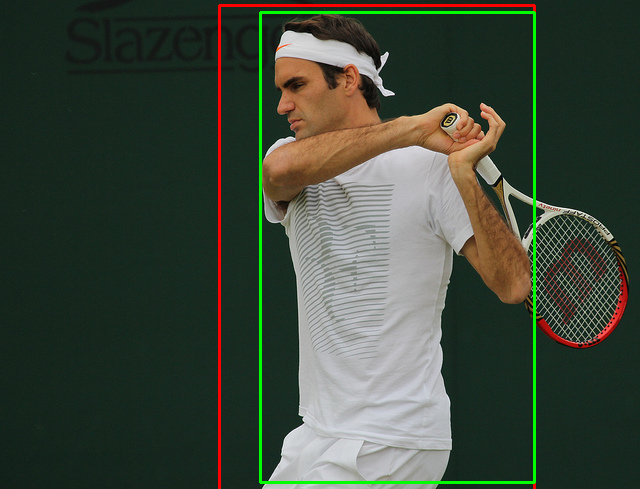
\includegraphics[width=11cm]{./imageDetectionCompareCOCO}
\caption{Comparación bounding boxes real y detectada con imagen de la BBDD COCO.}
\label{DetectionCompareCOCO}
\end{center}
\end{figure}

\section{Índice Jaccard}
\lhead[\thepage]{\thesection. Índice Jaccard}

El índice Jaccard, también conocido como \textbf{Intersection over Union}, es una estadística utilizada para comparar la similitud y la diversidad de conjuntos de muestras. Este índice mide la similitud entre conjuntos de muestras finitas y se define como el tamaño de la intersección dividido por el tamaño de la unión de los conjuntos de muestras.\\

\begin{equation}
J(A,B) = \frac{|A\cap B|}{|A\cup B|} = \frac{|A\cap B|}{|A| + |B| - |A\cap B|}
\end{equation}

\begin{figure}[H]
\begin{center}
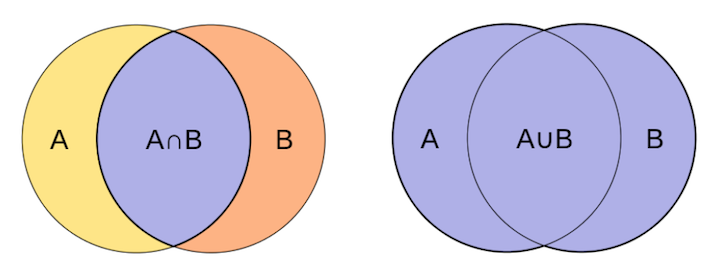
\includegraphics[width=11cm]{./Intersection&Union}
\caption{Intersección y unión sobre 2 conjuntos A y B.}
\end{center}
\end{figure}

Si no hay coincidencias en ambos conjuntos, el índice Jaccard se definirá como J(A,B) = 1.

\begin{equation}
0\leq J(A,B) \leq  1
\end{equation}
\\
Por lo tanto, el índice Jaccard o \textbf{Intersection over Union} (loU) se puede definir gráficamente de la siguiente manera:

\begin{figure}[H]
\begin{center}
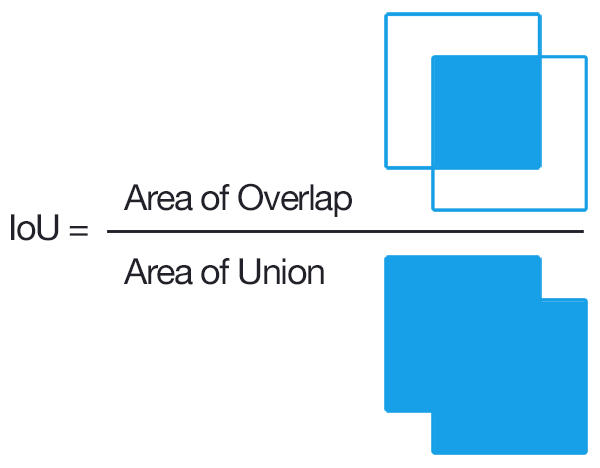
\includegraphics[width=8cm]{./loU}
\caption{Intersection over Union.}
\label{IntersectionOverUnion}
\end{center}
\end{figure}

Para determinar la calidad de un detector, se utilizarán la \textit{bounding box} real, obtenida de las anotaciones, y la \textit{bounding box} detectada, calculando de esta manera el índice Jaccard. Por lo tanto, podemos evaluar la calidad de un detector a partir del valor obtenido:

\begin{itemize}
\item Si el índice Jaccard tiene un valor alrededor de \textbf{0.4}, se considerará una calidad de detección escasa.
\item Si el índice Jaccard tiene un valor alrededor de \textbf{0.7}, se considerará una calidad de detección buena.
\item Si el índice Jaccard tiene un valor alrededor de \textbf{0.9}, se considerará una calidad de detección excelente.
\end{itemize}

\begin{figure}[H]
\begin{center}
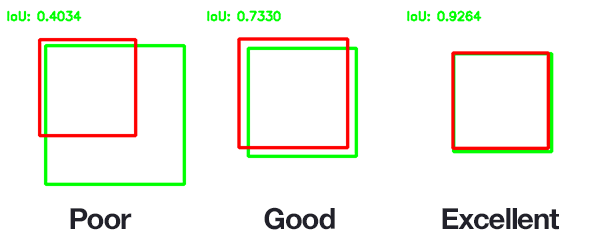
\includegraphics[width=11cm]{./loU_score}
\caption{Evaluación loU.}
\end{center}
\end{figure}


\section{Cálculo del índice Jaccard}
\lhead[\thepage]{\thesection. Calculo del índice Jaccard}

Se partirá de los \textit{scripts} explicados en los apartados \ref{ComparePascalVOC} y \ref{CompareCOCO} pero ahora los scripts crearán un fichero mostrando el índice Jaccard calculado para cada uno de los objetos de las 2 bases de datos. Estos 2 nuevos \textit{scripts}, a diferencia de los anteriores, recibirán un conjunto de imágenes, por lo que el primer paso para realizarlos será preparar los datos de entrada.\\

\begin{itemize}
\item Para el script que evaluará las imágenes de la base de datos PascalVOC, utilizaremos la ruta a las imágenes y a los ficheros de anotaciones. A partir de esto, se crearán 2 variables las cuales contendrán un listado con todos los archivos.\\

\begin{lstlisting}[frame=single]
dirsImages = sorted(os.listdir(pathImages))
dirsAnnotations = sorted(os.listdir(pathAnnotations))
\end{lstlisting}

Posteriormente, se iniciará un bucle en el que se llamará a la función \textit{detectiontest} tantas veces como se desee.\\

\begin{lstlisting}[frame=single]
for x in range(len(dirsImages)):
    if x == 200:
        break
    image = cv2.imread(pathImages + dirsImages[x])
    img_gray = cv2.cvtColor(image, cv2.COLOR_BGR2GRAY)
    img_rgb = cv2.cvtColor(img_gray,cv2.COLOR_GRAY2RGB)
    detec = net.detectiontest(image,
    					pathAnnotations + dirsAnnotations[x])
    detec_array.append(detec)
\end{lstlisting}

A esta función se le pasará como parámetro la imagen de entrada y su ruta y devolverá el índice Jaccard obtenido para cada uno de los objetos de la imagen de entrada. Después, introducirá estos valores en la variable \textit{detec\_array}.\\

\item Para el script que evaluará las imágenes de la base de datos COCO, la única diferencia será que solo habrá que listar la carpeta donde se encuentran las imágenes. En esta base de datos existe un único fichero de anotaciones que contiene todos los datos reales de cada una de las imágenes de ella por lo que no será necesario asociar cada imagen a un fichero de anotaciones. Posteriormente, se llamará al bucle de la misma manera que se ha comentado en el punto anterior.
\end{itemize}

Con los \textit{scripts} explicados en los apartados \ref{ComparePascalVOC} y \ref{CompareCOCO} tenemos disponibles las \textit{bounding boxes} reales y detectadas necesarias para calcular el índice Jaccard. Ahora, los 2 nuevos \textit{scripts} creados no pintarán estas cajas delimitadoras dentro de la imagen si no que las utilizarán para calcular el índice. Para ello, se crearán 4 nuevas funciones, las cuales se explican a continuación.\\ 

La primera de ellas se llamará \textit{area}, la cual recibirá un array con las coordenadas de los rectángulos sobre los cuales se quiere conocer su área y devolverá un array con los valores obtenidos.\\

\begin{lstlisting}[frame=single]
    def area(self, array_positions):
        area_array = []
        for i in range(len(array_positions)):
            weight = float(array_positions[i][2]) - 
            		float(array_positions[i][0])
            height = float(array_positions[i][3]) -
            		float(array_positions[i][1])
            area = weight * height
         
            area_array.append(area)
            
        return area_array
\end{lstlisting}

A esta función se la llamará 2 veces, guardando los valores obtenidos en las variables \textit{truth\_area} y \textit{detection\_area} las cuales se referirán al area de las \textit{bounding boxes} reales y detectadas respectivamente.\\

El segundo método se llamará \textit{rectangle\_intersection} y se encargará de calcular las coordenadas del rectángulo que forman las \textit{bounding boxes} real y detectada cuando intersectan. Para ello, se le pasará como parámetro las coordenadas reales y detectadas para cada uno de los objetos localizados en la imagen. En esta función se realizarán varias comprobaciones con el objetivo calcular las coordenadas del rectángulo intersección.\\

\begin{itemize}
\item La coordenada \textit{xmin} del rectángulo intersección será la coordenada \textit{xmin} \textbf{mayor} de los 2 rectángulos que intersectan.\\
\begin{lstlisting}[frame=single]
if rectangles_array1[0][x][0]) >= rectangles_array2[x][0]:
	xmin_intersection = rectangles_array1[0][x][0]
else:
	xmin_intersection = rectangles_array2[x][0]
\end{lstlisting}
\item La coordenada \textit{ymin} del rectángulo intersección será la coordenada \textit{ymin} \textbf{mayor} de los 2 rectángulos que intersectan.\\
\begin{lstlisting}[frame=single]
if rectangles_array1[0][x][1] >= rectangles_array2[x][1]:
	ymin_intersection = rectangles_array1[0][x][1]
else:
	ymin_intersection = intrectangles_array2[x][1]
\end{lstlisting}
\item La coordenada \textit{xmax} del rectángulo intersección será la coordenada \textit{xmax} \textbf{menor} de los 2 rectángulos que intersectan.\\
\begin{lstlisting}[frame=single]
if rectangles_array1[0][x][2] <= rectangles_array2[x][2]:
	xmax_intersection = rectangles_array1[0][x][2]
else:
	xmax_intersection = rectangles_array2[x][2]
\end{lstlisting}
\item La coordenada \textit{ymax} del rectángulo intersección será la coordenada \textit{ymax} \textbf{menor} de los 2 rectángulos que intersectan.\\
\begin{lstlisting}[frame=single]
if rectangles_array1[0][x][3] <= rectangles_array2[x][3]:
	ymax_intersection = rectangles_array1[0][x][3]
else:
	ymax_intersection = rectangles_array2[x][3]
\end{lstlisting}
\end{itemize}

Finalmente, la función devolverá el array \textit{positions\_array} el cual contendrá un array con las coordenadas de cada uno de los rectángulos calculados anteriormente.\\

\begin{lstlisting}[frame=single]
positions = []
positions.append(xmin_intersection)
positions.append(ymin_intersection)
positions.append(xmax_intersection)
positions.append(ymax_intersection)
positions_array.append(positions)
\end{lstlisting}

Después de esto, se llamará a la función \textit{area}, explicada anteriormente, para obtener el área de los rectángulos intersección, creando así la variable \textit{area\_intersection}.

El último parámetro necesario para calcular el índice Jaccard, es el área total de la \textit{bounding box} real y detectado. Para ello, se utiliza el método \textit{area\_total}, el cual recibirá como parámetro las coordenadas reales y detectadas de cada \textit{bounding box}, y el área de los rectángulos intersección calculados anteriormente y almacenados en la variable \textit{area\_intersection}.\\

\begin{lstlisting}[frame=single]
def area_total(self, rectangle1, rectangle2, area_intersection):
\end{lstlisting}

Esta función recorrerá todos lo rectángulos asociados, calculando en primer lugar el área de cada uno de ellos.\\

\begin{lstlisting}[frame=single]
heigh_rectangle1 = rectangle1[0][x][3] - rectangle1[0][x][1]
weigh_rectangle1 = rectangle1[0][x][2] - rectangle1[0][x][0]
area_rectangle1 = heigh_rectangle1 * weigh_rectangle1

heigh_rectangle2 = rectangle2[x][3] - rectangle2[x][1]
weigh_rectangle2 = rectangle2[x][2]) - int(rectangle2[x][0]
area_rectangle2 = heigh_rectangle2 * weigh_rectangle2
\end{lstlisting}

El área total se calculará sumando el área total de los 2 rectángulos y eliminando posteriormente el área del rectángulo intersección, el cual se ha pasado a la función como parámetro. Por último, se agregará al array \textit{area\_total\_array} el valor obtenido.\\

\begin{lstlisting}[frame=single]
area_total=area_rectangle1+area_rectangle2-area_intersection[x]

area_total_array.append(area_total)
\end{lstlisting}

Tras realizar estos métodos, se dispondrán de todos los datos necesarios para el cálculo del índice Jaccard. Como se explica en el apartado \ref{IndiceJaccard} y se muestra gráficamente el la figura \ref{IntersectionOverUnion}, el índice Jaccard se calcula dividiendo la intersección de los 2 conjuntos entre la unión de ambos, es decir, el área del rectángulo intersección entre el área total. Para ello, se utilizará la función \textit{jaccard\_index} la cual recibirá como parámetro las variables \textit{area\_intersection} y \textit{area\_total}, que contienen los datos necesarios para el cálculo del índice.\\

\begin{lstlisting}[frame=single]
def jaccard_index(self, area_total, area_intersection):
\end{lstlisting}

Este método recorrerá un bucle cuya longitud será el total del conjunto de \textit{bounding boxes} reales y detectadas para cada objeto identificado, realizando la división comentada anteriormente. Finalmente, el resultado se devolverá en la variable \textit{jaccard\_index\_array}.\\

\begin{lstlisting}[frame=single]
jaccard_index = float(area_intersection[x]) / float(area_total[x])

jaccard_index_array.append(jaccard_index)
\end{lstlisting}

Una vez conseguido el valor del índice Jaccard, la función \textit{detectiontest} devolverá 2 arrays. El primero con el valor del índice Jaccard obtenido y el segundo con todas las etiquetas de los objetos detectados. Estos 2 arrays se pueden relacionar con el índice, ya que el valor del índice Jaccard en una determinada posición del array es el obtenido para el objeto existente en la misma posición del segundo array.\\

Como se ha comentado al principio de esta sección, ambos \textit{scripts}, tanto el que utiliza las imágenes de entrada de PascalVOC como el que utiliza las de COCO, llamarán a la función \textit{detectiontest} una vez por cada imagen de entrada, guardando el resultado obtenido en cada llamada al método en la variable \textit{detec\_array}.\\

Cuando se obtengan todos los valores del índice Jaccard que se desee, se generarán 2 ficheros, que mostrarán las estadísticas de los datos obtenidos. El primer fichero se llamará \textit{jaccardIndex.txt} y mostrará el índice Jaccard para cada uno de los objetos detectados en cada una de las imágenes. Para ello se recorrerá la variable \textit{detec\_array} relacionando los índices de éste.\\

\begin{lstlisting}[frame=single]
if detec_array[x][1][i] == "aeroplane":
	aeroplane_jaccard = aeroplane_jaccard + detec_array[x][0][i]
	naeroplane = naeroplane + 1
\end{lstlisting}

El código anterior comparará una variable creada con el nombre de una de las etiquetas de las base de datos con la etiqueta de cada objeto detectado, 

\section{Resultado final}
\lhead[\thepage]{\thesection. Resultado final}


\chapter{Conclusiones}
\markboth{CONCLUSIONES}{CONCLUSIONES}

En este capítulo se van a exponer las principales conclusiones obtenidas durante el desarrollo de este trabajo. Además, se propondrán varias líneas de trabajo futuras para continuar con la tarea realizada.

\section{Conclusiones}

El desarrollo de este trabajo ha permitido llegar a una serie de conclusiones relacionadas con el aprendizaje profundo utilizando redes neuronales artificiales entrenadas usando la herramienta Caffe. Las conclusiones serán expuestas siguiendo los \textit{sub-objetivos} expuestos en la sección \ref{Objetivos}.

\begin{description}
\item[Estudio de la plataforma Caffe]\hfill 
\vspace{5pt}
\\
La plataforma Caffe es una herramienta de gran utilidad para el trabajo con redes neuronales ya que el entrenamiento se ejecuta de una forma muy sencilla, además de aportar varios ejemplos para introducirse en el ámbito de la inteligencia artificial con los problemas de clasificación y detección. 
\item[Estudio de varias bases de datos aplicadas a la detección]
\item[Estudio de la técnica SSD]
\item[Desarrollo de un componente detector]\hfill 
\vspace{5pt}
\\
El componente Python desarrollado ofrece buenos resultados con las redes neuronales entrenadas previamente. El desacoplar la tarea en 3 hilos, dedicando uno únicamente al proceso de detección, hace que la aplicación sea más robusta evitando que ésta baje su rendimiento debido a la detección, ya que se realiza a la velocidad que pueda soportar la CPU del equipo utilizado.
\item[Cálculo del \textit{índice Jaccard} o \textit{Intersection Over Union}]\hfill 
\vspace{5pt}
\\
El \textit{índice Jaccard} o \textit{Intersection Over Union} es un parámetro de gran utilidad para conocer las prestaciones y eficacia de una red neuronal entrenada. Gracias a él, se pueden comparar fácilmente varias redes neuronales con el objetivo de hacerlas más robustas.
\end{description}

\section{Líneas futuras}

Tras la exposición de las conclusiones, se enumeran varias líneas de investigación que ayudarían a continuar con lo desarrollado durante este trabajo.

\begin{itemize}
\item Una línea de investigación cercana a la abordada sería la de detección de objetos utilizando algunos de los softwares adicionales para redes neuronales explicados en el apartado \ref{SoftwaresRNN}.
\item
\end{itemize}

\begin{thebibliography}{X}
\addcontentsline{toc}{chapter}{Bibliografía}

\bibitem{IA_Introduccion}
Wei Di, Anurag Bhardwaj, Jianing Wei
\newblock {Deep Learning Essentials. Your hands-on guide to the fundamentals of deep learning and neural network modeling}

\bibitem{IA_Encyclopedia}
John Wiley \& Sons.
\newblock {Encyclopedia of Artificial Intelligence}

\bibitem{IA}
Raúl Pino Diez, Alberto Gómez Gómez, Nicolás de Abajo Martínez.
\newblock {Introducción a la Inteligencia Artificial. Sistemas expertos, redes neuronales artificiales y computación evolutiva}
\newblock {Noviembre 2003}

\bibitem{IA_2}
Francisco Escolano, Miguel Ángel Cazorla, María Isabel Alfonso, Otto Colomina y Miguel Ángel Lozano.
\newblock {Inteligencia Artificial: Modelos, Técnicas y Áreas de Aplicación}
\newblock {Noviembre 2003}

\bibitem{ML}
Aprendizaje automático.
\newblock {\url{https://es.wikipedia.org/wiki/Aprendizaje_autom%C3%A1tico}}

\bibitem{CancerMamaDeepLearning}
D.~{Wang}, A.~{Khosla}, R.~{Gargeya}, H.~{Irshad}, and A.~H. {Beck}.
\newblock {Deep Learning for Identifying Metastatic Breast Cancer}.
\newblock {\em ArXiv e-prints.}, June 2016.

\bibitem{NeuronaModelo}
La predicción del dato: Redes Neuronales Artificiales.
\newblock {\url{https://www.analiticaweb.es/la-prediccion-del-dato-redes-neuronales-artificiales/}}

\bibitem{CapasRNA}
Jordi Torres.
\newblock {Deep Learning - Introducción práctica con Keras}
\newblock {\url{https://jorditorres.org/redes-neuronales-densamente-conectadas/}}

\bibitem{CNN}
DEWI SURYANI, S.KOM., M.ENG.
\newblock {CONVOLUTIONAL NEURAL NETWORK, \textit{Binus University - School of Computer Science.}}
\newblock {\url{http://socs.binus.ac.id/2017/02/27/convolutional-neural-network/}}

\bibitem{SSD_3}
Deep Learning.
\newblock{Deep Learning (Aprendizaje profundo). Tres cosas que es necesario saber}.
\newblock {\url{hhttps://es.mathworks.com/discovery/deep-learning.html}}

\bibitem{RNN}
Edgar Nelson Sánchez Camperos y Alma Yolanda Alanís García.
\newblock {Redes Neuronales: Conceptos fundamentales y aplicaciones a control automático}

\bibitem{TiposCapasRNA}
Pedro Larrañaga, Iñaki Inza, Abdelmalik Moujahid. Departamento de Ciencias de la Computación e Inteligencia Artificial. Universidad del País Vasco?Euskal Herriko Unibertsitatea.
\newblock {Tema 8. Redes Neuronales}
\newblock {\url{http://www.sc.ehu.es/ccwbayes/docencia/mmcc/docs/t8neuronales.pdf}}


\bibitem{SSD}
Wei Liu ,Dragomir Anguelov, Dumitru Erhan, Christian Szegedy, Scott Reed , Cheng-Yang Fu, Alexander C. Berg.
\newblock {Single Shot MultiBox Detector}


\bibitem{SSD_2}
Single Shot MultiBox Detection.
\newblock{Understanding SSD MultiBox? - ?RealTime Object Detection In Deep Learning}.
\newblock {\url{https://towardsdatascience.com/understanding-ssd-multibox-real-time-object-detection-in-deep-learning-495ef744fab}}



\end{thebibliography}

\end{document}